% !Mode:: "TeX:UTF-8"
%!TEX program  = xelatex

%\documentclass[bwprint,fontset=windows]{gmcmthesis}
\documentclass[bwprint]{gmcmthesis}
\usepackage{listings}
\lstset{
    language=Python,
    basicstyle=\ttfamily,
    numbers=left,
    numberstyle=\tiny,
    breaklines=true,
    frame=single,
    keywordstyle=\color{blue},     % 关键字的颜色为蓝色
    commentstyle=\color{green},   % 注释的颜色为绿色
    stringstyle=\color{red},      % 字符串的颜色为红色
    morekeywords={new_keyword1, new_keyword2} % 添加额外的关键字
}



\hypersetup{hidelinks}
\usepackage[framemethod=TikZ]{mdframed}

%\usepackage{fontspec}  % for Consolas & Courier New
%\lstset{basicstyle=\small\fontspec{Consolas}}
%\lstset{basicstyle=\small\fontspec{Courier New}}
%\setmonofont{Consolas}
%\setcounter{tocdepth}{3}   % 调整目录深度

\usepackage{subfig}
\usepackage{colortbl}
\usepackage{booktabs}
\definecolor{color1}{rgb}{0.78,0.88,0.99}
\definecolor{color2}{rgb}{0.36,0.62,0.84}
%\definecolor{color3}{rgb}{0.8235,0.8706,0.9373}
\definecolor{color3}{rgb}{0.88,0.92,0.96}
\definecolor{color4}{rgb}{0.96,0.97,0.98}%{0.9176,0.9373,0.9686}

% 算法
\usepackage[noend]{algpseudocode}
\usepackage{algorithmicx,algorithm}
\floatname{algorithm}{算法}
\renewcommand{\algorithmicrequire}{\textbf{输入:}}
\renewcommand{\algorithmicensure}{\textbf{输出:}}

%\numberwithin{equation}{section}
%\numberwithin{figure}{section}
%\numberwithin{table}{section}


\newcommand{\red}[1]{\textcolor{red}{#1}}
\newcommand{\blue}[1]{\textcolor{blue}{#1}}


%===================== 建模论文题目 ======================

\title{脑出血患者预测模型的构建与评估}
\baominghao{\hspace{6em} xxxxxx} %参赛队号
\schoolname{\hspace{5.8em} School} %学校名称
\membera{\hspace{6em} A} %队员A
\memberb{\hspace{6em} B} %队员B
\memberc{\hspace{6em} C} %队员C

%=======================================================


\begin{document}

%生成标题
\maketitle

%填写摘要
\begin{abstract}
出血性脑卒中是由非外伤性脑内血管破裂引起的脑出血。其病因复杂,常由脑动脉瘤破裂、脑动脉异常等导致血液涌入脑组织,造成机械性损伤。血肿范围扩大是预后不良的重要危险因素之一,需要监测和控制血肿扩张。血肿周围水肿可能导致脑组织受压,进一步损伤神经功能。因此,建立智能诊疗模型,明确导致出血性脑卒中预后不良的危险因素,实现精准个性化的疗效评估和预后预测具有重要意义。\par
针对出血性脑卒中的医学影像数据化分析问题,我们在对患者信息原始数据进行匹配处理和统计分析的基础上,构建了多种预测模型,包括LightGBM和随机森林结合的分类预测模型、混合线性预测和BiLSTM结合的混合预测模型、基于K-Means的聚类模型,以及基于两独立样本t检验的因果推断模型。我们使用python编程对全体患者进行亚组聚类,预测各个患者发生血肿扩张事件的概率;同时探究血肿体积、水肿体积和不同治疗方式之间的内在联系;最后,我们预测患者预后90天的mRS评分,并分析出血性脑卒中患者的预后90天mRS评分与个人史、疾病史、治疗方法及影像特征等之间的关联关系,并依此为临床相关决策提供建议。\par
针对问题一,分析患者的入院首次影像检查时间间隔和 $HM\_volume $数据,以确定是否发生了血肿扩张事件,首先需要对原始数据进行预处理。本问通过pandas库对原始附件中的表格信息进行匹配与合并,并将发病到首次影像检查的时间间隔与首次影像检查的时间点进行加和,从而确定真正的发病间隔,以此判断患者是否在48小时内发生了血肿扩张事件。其次,我们借助Nelder-Mead算法将LightGBM和随机森林模型结合,并使用VotingClassifier集成学习器,通过采用不同的算法和数据特征,降低过拟合风险,提高模型的泛化能力,并获得了更可靠的预测结果。经检验,集成后的模型对患者发生血肿扩张事件概率的预测精度达到了 99\%,相较集成之前的单一模型,误差下降了 70\%。所有患者样本的血肿扩张情况和发生概率预测值记录在表4中。\par
针对问题二,我们借助CEEMD模态分解的功能将混合线性预测模型和BiLSTM相结合,研究了血肿周围水肿的发生及进展血肿周围水肿的发生及进展,分别对各患者水肿体积的初始大小,以及水肿体积的相对大小随时间的变化进行预测,得到模型对患者水肿体积大小和发病时间间隔拟合曲线的RMSE为25670.456。其次,我们通过feature importance对影响患者水肿体积大小的特征进行评估,选取前十名影响最大的特征作为K-Means的聚类依据,实现了对患者的亚组划分。结果表明,当聚类数为4时,模型对患者水肿体积大小随时间进展的拟合残差RMSE最小,为15740.167,相较于聚类前性能提升了36.6\%。接着,我们建立了基于两独立样本t检验的因果推断模型,对不同治疗方法对水肿体积进展模式的影响进行分析,得出结论:1.脑室引流组和对照组之间存在显著差异,p 值非常小(0.00025),T 统计量为负值(-3.7664),平均数差为正值(11.9008),即脑室引流治疗可以有效降低水肿体积的大小;2.止血治疗可能会导致轻微的增加患者水肿体积的大小,p 值较小(0.00527),T 统计量为正值(2.83855),平均数差为负值(-5.46171)。最后,在研究血肿体积、水肿体积及治疗方法三者间的关系时,我们沿用第二小问中设立的患者亚组类别,并借助时间序列相关性分析模型与因果推断模型分别对血肿体积和水肿体积的关系、血肿体积和治疗方法的关系以及水肿体积和治疗方法的关系进行分析。\par
针对问题三,为了预测患者90天的mRS评分,需要先对患者的个人史、疾病史、发病相关及首次影像结果等特征进行one-hot编码,并将连续特征归一化到[0,1]范围,然后使用深度森林模型对mRS评分进行预测,经检验模型二次拟合后的训练精度达到了0.87。接着,为了预测含随访影像检查的患者90天的mRS评分,我们在数据处理阶段加入了时间间断来引入时间因素,并借助LSTM模型mRS评分进行预测,经检验模型二次拟合的训练精度达到了0.995。最后,我们借助pearson相关性分析和feature importance模型对出血性患者的预后与其个人史、疾病史、治疗方法以及影像特征之间的关系进行了探究。结果表明,对血性脑卒中患者的预后90天mRS评分影响最大的特征前几名分别为:糖尿病史、右前动脉血肿分布比例和发病到影像时间间隔。\par
综上,本文针对出血性脑卒中的医学影像数据化分析问题,通过构建多种智能诊疗模型,包括预测血肿扩张事件概率、水肿体积及其进展模式的预测、预测患者90天的mRS评分,并探究出血性脑卒中预后与个人史、疾病史、治疗方法和影像特征等的关系。本研究的成果对于实现精准个性化的疗效评估和预后预测具有重要的现实意义,可以为出血性脑卒中的临床决策提供科学依据。


\keywords{医学影像数据化分析\quad  深度森林\quad   BiLSTM\quad  LightGBM}

\end{abstract}

\pagestyle{plain}

%目录 不推荐加
\maketoc

\clearpage

\section{问题重述}

\subsection{引言}   % 问题的背景

出血性脑卒中是由非外伤性脑内血管破裂引起的脑出血\cite{李立新2010缺血性和出血性脑卒中危险因素分析},占脑卒中病例的10-15\%。其病因复杂,通常源于脑动脉瘤破裂、脑动脉异常等因素,导致血液流入脑组织,引发脑部机械性损伤和生理病理反应。出血性脑卒中具有急性起病和快速进展的特点,其急性期病死率高达45-50\%,大多数患者伴有神经功能障碍,给社会和家庭带来沉重的负担。因此,准确评估其发病风险、精准预测患者的预后,以优化临床决策,显得至关重要。

血肿范围扩大是出血性脑卒中不良预后的一个重要危险因素\cite{黄广苏2009脑出血早期血肿扩大的研究进展,吴智平2004脑出血后血肿扩大}。血肿范围可能由脑组织受损和炎症逐渐扩大,导致颅内压力急剧上升,进一步损害神经功能,甚至危及生命。因此,监测和控制血肿扩张成为临床关注的焦点之一。同时,血肿周围水肿也备受关注,它可能导致脑组织受到压迫,影响神经元功能,加重神经功能损伤。因此,早期发现和预测血肿扩张和周围水肿对于患者的预后至关重要。

医学影像技术和人工智能为监测脑组织损伤提供了强大的工具\cite{徐凤霞1996医学影像新技术在脑血管病诊断中的应用,李如画2018医学影像在诊断过程中的作用}。因此,利用人工智能技术深度分析影像数据,结合个体信息、治疗方案和预后数据,构建智能诊疗模型,明确不良预后的危险因素,实现精确评估和预测引起了医疗界的广泛关注。



\subsection{问题的提出}

%\subsubsection{问题的提出内容一}

\noindent 围绕出血性脑卒中临床智能诊疗的建模工作,本文依次提出如下问题:
\subsubsection{问题一}
\textbf{a:} 基于给定的数据表格"表1"和"表2",针对患者sub001至sub100,分析各患者入院首次影像检查时间间隔和HM\_volume数据,确定患者在发病后的48小时内是否发生了血肿扩张事件。若发生了血肿扩张事件,需记录事件发生的时间,并将结果填写到"表4"中的相应字段。


\textbf{b:} 基于给定的前100例患者(sub001至sub100)的个人信息、疾病史以及与发病相关的信息,以及这些患者首次影像检查结果,构建一个预测模型来预测所有患者(sub001至sub160)是否在发病后发生血肿扩张事件。同时,借助建立的预测模型估计每位患者发生血肿扩张的概率,从而降低早期识别患者的风险,以便于采取适当的医疗干预措施。

\subsubsection{问题二}
\textbf{a:} 使用前100个患者的水肿体积数据和相关重复检查时间点,以建立描述水肿体积随时间变化的数学模型。使用建立好的数学模型将用于拟合患者的实际水肿体积数据。随后,需要计算实际水肿体积值与模型预测值之间的残差,以评估模型的准确性。这个任务的完成,有助于了解水肿随时间的动态变化,为进一步的研究提供基础数据。


\textbf{b:} 在此任务中,需要研究不同患者在水肿体积随时间变化方面的个体差异。首先,将患者分为3至5个亚组,每个亚组代表一组具有相似水肿体积随时间变化模式的患者。随后,为每个亚组构建水肿体积随时间变化的曲线,以捕捉不同亚组之间的模式差异。接着,需要计算前100位患者的实际水肿体积值与其所属亚组曲线预测值之间的残差。最后,记录患者所属的亚组信息以及计算得到的残差结果,并将它们填写在规定的表格位置。这个任务有助于深入了解不同患者群体之间水肿体积随时间变化的差异,同时为个体化治疗提供重要见解。


\textbf{c:} 在此任务中,需要分析不同治疗方法对水肿体积进展模式的影响。具体而言,研究将基于患者的治疗方案,即“表1”字段Q至W中的信息,来评估治疗方法对水肿体积的影响程度。这个分析旨在揭示不同治疗方法是否对水肿的发展模式产生显著影响,以及不同治疗方法之间可能存在的差异。这个研究有助于为患者提供更个性化的治疗建议,以优化脑水肿的管理和治疗策略。


\textbf{d:} 在此任务中,需要分析血肿体积、水肿体积以及不同治疗方法(“表1”字段Q至W)之间的关系。具体而言,研究将调查这三个因素之间是否存在相关性或相互影响。这种分析有助于深入了解不同治疗方法如何影响血肿和水肿的体积,并探究它们之间的关联,以便更好地理解脑部损伤的发展和治疗效果。这项研究有助于为医护人员提供有关最佳治疗方法和策略的重要见解,以实现更好的临床管理和患者护理。


\subsubsection{问题三}
\textbf{a:} 在此任务中,需要基于前100位患者的个人史、疾病史、发病及治疗相关特征以及首次影像检查结果构建一个预测模型,用于预测所有患者在发病后90天的mRS评分。这个预测模型将考虑患者的首次影像数据,并旨在提供对患者预后的有用信息。预测结果将以有序等级变量(0-6)的形式记录,并填写在“表4”的I字段中。


\textbf{b:} 本任务要求利用前100位患者的全部临床、治疗信息以及首次和随访影像结果构建一个预测模型,用于预测所有具有随访影像检查的患者在发病后90天的mRS评分。这个模型将综合考虑患者的多方面信息,以提供更准确的预测结果。预测结果将以有序等级变量(0-6)的形式记录,并填写在“表4”的J字段中。


\textbf{c:} 在这个任务中,需要分析出血性脑卒中患者的90天mRS评分与其个人史、疾病史、治疗方法以及影像特征之间的关系。具体而言,研究将探讨这些因素与患者预后之间的相关性,以提供有关临床决策的建议。这项分析旨在帮助医疗专业人员更好地理解预后因素,并为患者提供更加个性化的治疗方案。

%\clearpage
%\section{问题分析}


\clearpage
\section{模型的假设}

\begin{enumerate}
\item 假设患者自身携带的其他疾病不会对被研究对象(血肿体积、水肿体积)造成影响;
\item 假设患者除已给出的身体信息外,其余身体状况不具有显著差异;
\item 假设不同治疗方法对患者起到的作用程度近似相等;
\item 假设患者在被研究过程中,不会因其他因素导致身体情况的骤变。
\end{enumerate}



\section{符号说明}

\begin{table}[htp!]
\centering
\renewcommand\arraystretch{1.2} %定义表格高度
\newcolumntype{L}{>{\quad}X}
\newcolumntype{P}[1]{>{\centering\arraybackslash}p{#1}}
\newcolumntype{C}{>{\centering \arraybackslash}X}
\newcolumntype{R}{>{\raggedright \arraybackslash}X}
\begin{tabularx}{0.9\textwidth}{P{3cm}|L}
   \toprule[1.2pt]
  符号    &   \quad 意义 \\
  \midrule %\midrule
  %\rowcolor[gray]{0.90}
  $ F $  &  回归树的空间    \\
  
  $ f_k $  &  相互独立的不同结构的树    \\
  
  $ c^{K-1} $  &  前 K − 1次棵树的正则化项和    \\
  
  $ l $  &  损失函数    \\
  
  $ \Omega $  &  惩罚函数     \\
  
  $ \beta $  &  固定效应的系数向量    \\
  
  $ \gamma $  &  随机效应的系数向量     \\
  
  $ \theta $  &  随机效应的系数向量     \\
  
  $ ReLU $  &  激活函数     \\
  

  $ learning\_rate $  &  学习率     \\
  
  $ ACF $  &  自相关函数    \\
  
  $ PACF $  &  偏自相关函数    \\
  
 \bottomrule[1.2pt]
\end{tabularx}
\end{table}


%\begin{tabularx}{\textwidth-18pt}{XXX}
%\hline
%Input & Output& Action return \\
%\hline
%DNF &  simulation & jsp\\
%\hline
%\end{tabularx}

\clearpage
\section{问题一建模与求解}
\subsection{问题分析}
本问一共包含两个小问,第一问需要根据表1和表2的数据,判断患者sub001至sub100发病后48小时内是否发生血肿扩张事件,并记录血肿扩张发生时间。第二问则需要以是否发生血肿扩张事件为目标变量,基于表1、表2和表3的数据,构建模型预测所有患者(sub001至sub160)发生血肿扩张的概率。

\subsection{第一问数据处理}
为了分析患者的入院首次影像检查时间间隔和HM\_volume数据,以确定是否发生了血肿扩张事件,我们首先需要对原始数据进行预处理。这个过程包括以下步骤:\\
{\bf 质量检测:}
首先,对原始数据进行严格的质量检测,以查找是否存在患者信息中的异常值或缺失值。\\
{\bf 数据合并:}
接着,使用pandas库的merge()函数来合并表1和表2中具有相同ID的患者信息。这一步骤有助于整合不同数据源的信息,以便进一步分析。\\
{\bf 列合并:}
最后,将患者信息中包含"流水号"字符串的列值及其之后的所有列值合并到对应的第一个索引行下。这样做可以实现对同一患者多次影像检查信息的合并,使数据更加整洁和易于分析。预处理后的表格部分展示如表\ref{tab:partly_display}:

\begin{table}[ht]
    \caption{预处理后部分数据展示}
    \centering
    \fontsize{10}{9}\selectfont
\renewcommand\tabcolsep{5pt}
{
    \begin{tabular}{cccccc}
    \toprule[1.2pt]
    \textbf{ID} & \textbf{首次检查流水号} & \textbf{HM\_volume} & \textbf{…} & \textbf{ED\_Cerebellum\_L\_Ratio} & \textbf{检查时间}       \\ \midrule
    sub001      & 20161212002136   & 69714               & …          & 0                                 & 2016-12-12 23:32:54 \\
    sub001      & 20161213000009   & 74902               & …          & 0                                 & 2016-12-13 05:19:00 \\
    sub001      & 20161218000100   & 70952               & …          & 0                                 & 2016-12-18 09:09:24 \\
    sub001      & 20161223001020   & 62831               & …          & 0                                 & 2016-12-23 16:47:09 \\
    …           & …                & …                   & …          & …                                 & …                   \\
    sub159      & 20200219000588   & 126642              & …          & 0                                 & 2020-02-19 15:01:00 \\
    sub160      & 20200821002584   & 49019               & …          & 0                                 & 2020-08-21 22:32:00 \\
    sub160      & 20200822000947   & 100470              & …          & 0                                 & 2020-08-22 12:01:00 \\ 
    \bottomrule[1.2pt]
    \end{tabular}}
    \label{tab:partly_display}
\end{table}


这些预处理步骤为我们提供了高质量的数据,以便进一步探索和分析患者的血肿扩张事件。

\subsection{第一问求解}
为了判断前100名患者是否在发病48小时内发生血肿扩张时间,并记录发生血肿扩张时间的时间,我们选择使用python的pandas库对预处理过后的数据进行进一步加工。患者血肿扩张情况的检测流程如图\ref{fig:1a解题思路}所示。

首先,使用Pandas读取预处理后的包含患者的临床信息和影像数据的数据集。接下来,编写query\_databas函数,从数据集中查询特定患者的血肿体积和检查时间信息,并进行患者ID的匹配。接着,创建get\_volumes函数,获取指定患者的血肿体积、检查时间以及发病到首次影像检查的时间间隔。然后,编写check\_expanded函数,检查特定患者是否在发病后48小时内发生血肿扩张事件。通过check\_expanded函数计算血肿体积的变化和时间间隔,如果满足条件(即血肿扩张),则会记录扩张事件发生的时间和相关信息。接着,通过迭代遍历预处理后表格中的患者数据,对每个患者进行查询和血肿扩张的检查,然后将结果填充到答案文件中的相应位置,以便进行进一步的分析和报告。

需要注意的是,患者在发病到首次影像检查之间具有一定的时间间隔,会影响到48小时内发生血肿扩张事件的判定。因此,在对同一患者多次检查时间间隔进行计算时,需加上发病到首次影像检查的时间间隔,以保证血肿扩张时间判定的准确性。

\begin{figure}[h]
    \centering
    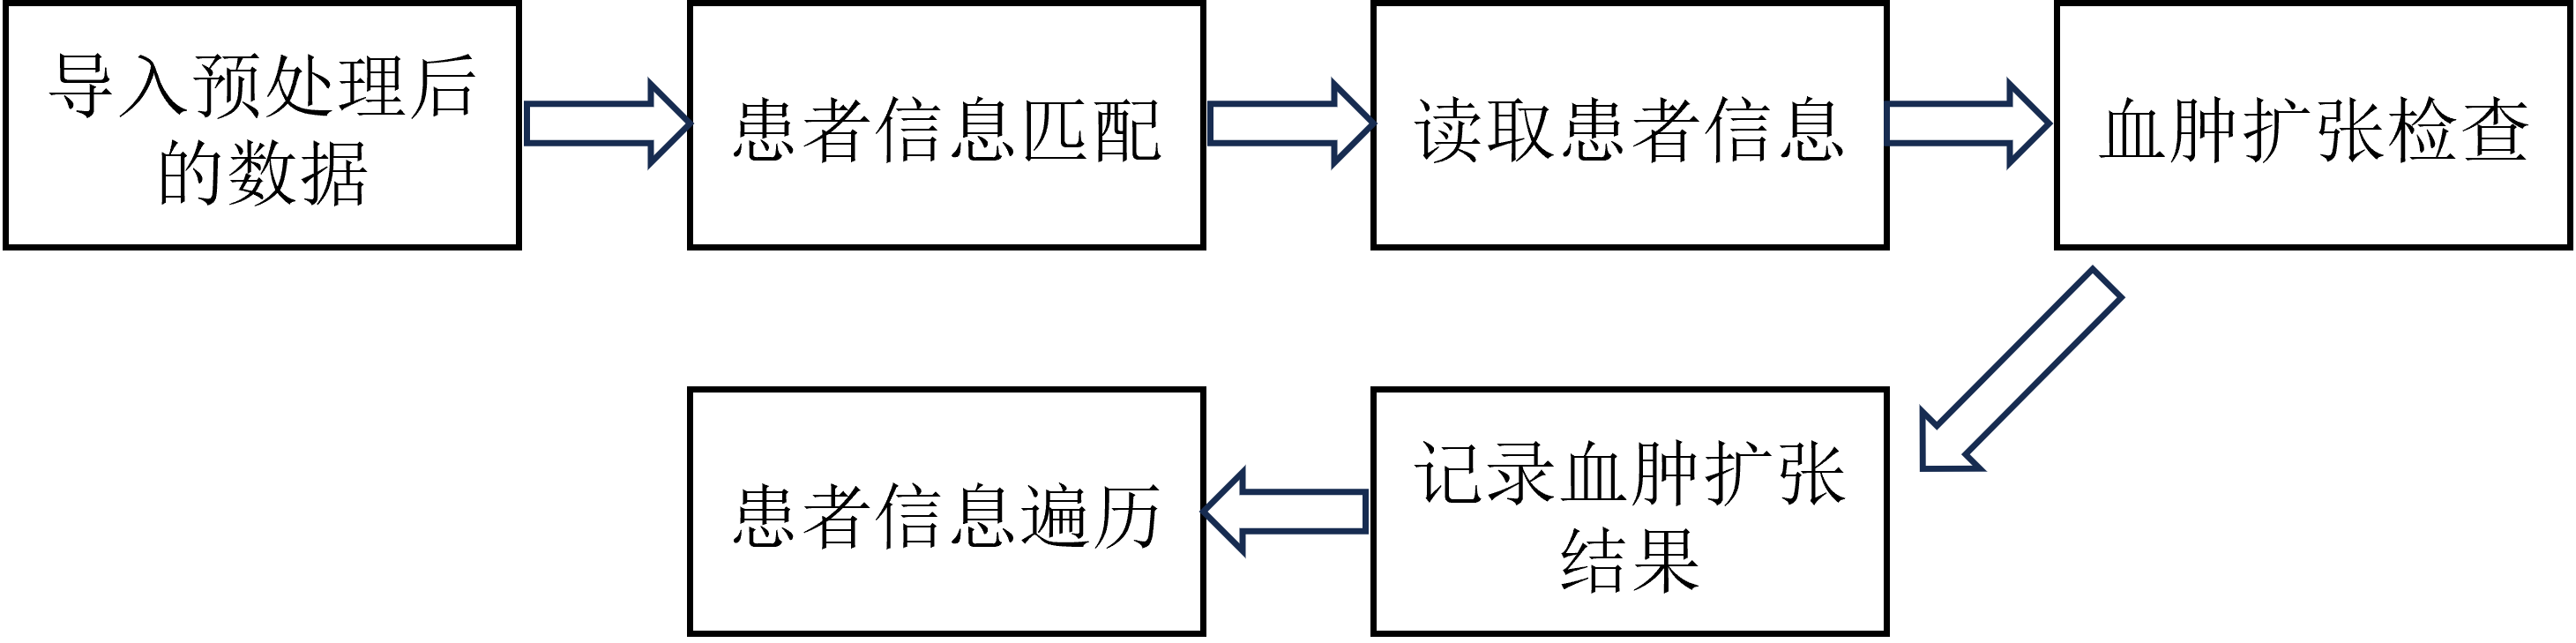
\includegraphics[width = \linewidth]{figures/1a解题思路.png}
    \caption{血肿扩张检测流程}
    \label{fig:1a解题思路}
\end{figure}

至此,我们通过整合和分析患者的临床信息和影像数据,成功地完成了预测患者是否在发病后48小时内发生血肿扩张事件的任务,并记录了相关的结果,为临床问题的解决提供了有力支持。

\subsection{第二问模型建立与求解}
在本问中,我们的目标是基于前100例患者的个人史、疾病史、发病及治疗相关特征、首次影像检查结果等变量,构建一个模型,以预测所有患者(sub001至sub160)是否会发生血肿扩张事件,并输出患者发生血肿扩张事件的概率。\par
\subsubsection{模型介绍}

\paragraph{LightGBM模型} 
\paragraph{\hspace{3em}}Light Gradient Boosting Machine (LightGBM)是一种梯度提升树(Gradient Boosting Tree)算法的改进版本,它具有高效的训练速度和优秀的性能。与传统的梯度提升树不同,LightGBM引入了创新性的设计和优化,以提高模型的效率和泛化能力\cite{ke2017lightgbm},其基本原理为:

\begin{enumerate}
    \item Leaf-wise生长策略:使用以叶子数为导向(带深度限制的 Leaf-wise 算法)的决策树建立算法而不是大多数GBDT工具使用的决策树深度导向(按层生长 (level-wise) )的生长策略,可以降低误差,得到更好的精度。
    \item 分类特征的编码方式的优化:LightGBM使用直方图来加速特征的分裂计算。它将数据按照特征进行分桶,然后在分桶上进行分裂选择,避免了对所有数据点的排序操作,提高了训练速度。
\end{enumerate}

LightGBM通过不断增加扩充树模型,根据数据特征来分裂生长树,并拟合上次的预测残差,最后累加每颗树所得的预测值,即得到最后的预测结果:
\begin{equation}
\begin{aligned}
\hat{y}_i=\sum_{i=1} f_k\left(x_i\right), f_k \in F
\end{aligned}
\label{equ:1}
\end{equation}

式中,$F$表示回归树的空间,每个$f_k$分别代表相互独立的不同结构的树。
训练的目标函数如下式所示,其中$y_i$为标签真实值,$\hat{y}_i^{k-1}$为第$K-1$次学习结果,$c^{K-1}$为前$K-1$次棵树的正则化项和,目标函数的含义为寻找一颗合适的数$f_k$使得函数的值最小。

\begin{equation}
\begin{aligned}
\mathrm{obj}^K=\sum_i l\left(y_i, \hat{y}_i^K\right)+\Omega\left(f_k\right)+c^{K-1}=\sum_i l\left(y_i, \hat{y}_i^{K-1}+f_K\left(x_i\right)\right)+\Omega\left(f_k\right)+c^{K-1}
\end{aligned}
\label{equ:2}
\end{equation}

其中,$l$表示损失函数,表示预测值与真实值之间的残差,损失函数则是将每一棵树的残差相加,$\Omega$为惩罚函数。对于损失函数,可以拆分为每棵树的预测值与真实值的差值,假定第0课树为:$\hat{y}_i^0=0$。那么在构造第一颗树的时候,可以看成第0棵树的残差与第一颗树的残差相加,可以表示为:
\begin{equation}
\begin{aligned}
\hat{y}_i^1=\hat{y}_i^0+f_1\left(x_i\right)
\end{aligned}
\label{equ:3}
\end{equation}

因此构造第$K$棵树的时候,预测值可以表示为:
\begin{equation}
\begin{aligned}
\hat{y}_i^k=\hat{y}_i^{k-1}+f_k\left(x_i\right)
\end{aligned}
\label{equ:4}
\end{equation}

最终的损失函数可以表示为:
\begin{equation}
\begin{aligned}
\sum_i l\left(y_i, \hat{y}_i^k\right)=\sum_i l\left(y_i, \hat{y}_i^{k-1}+f_k\left(x_i\right)\right)
\end{aligned}
\label{equ:5}
\end{equation}

接下来运用泰勒展开,此时选择二阶展开式结果比较好,可以在保证精度的同时简化计算,损失函数的泰勒二阶展开为:
\begin{equation}
\begin{aligned}
\sum_i l\left(y_i, \hat{y}_i^{K-1}+f_K\left(x_i\right)\right)=\sum_i\left[l\left(y_i, \hat{y}_i^{K-1}\right)+g_i f_K\left(x_i\right)+\frac{1}{2} h_i f_K^2\left(x_i\right)\right]
\end{aligned}
\label{equ:6}
\end{equation}

$g_i$和$h_i$是与变量无关的常数,分别表示第$i$个样本损失函数的一阶偏导和二阶偏导:
\begin{equation}
\begin{aligned}
g_i=l^{\prime}\left(y_i, \hat{y}_i^{K-1}\right), h_i=l^{\prime \prime}\left(y_i, \hat{y}_i^{K-1}\right)
\end{aligned}
\label{equ:7}
\end{equation}

简化后的目标函数可表示为:
\begin{equation}
\begin{aligned}
\mathrm{obj}^K=\sum_i\left[L\left(y_i, \hat{y}_i^{K-1}\right)+g_i f_K\left(x_i\right)+\frac{1}{2} h_i f_K^2\left(x_i\right)\right]+\Omega\left(f_K\right)+c
\end{aligned}
\label{equ:8}
\end{equation}

\paragraph{随机森林模型} 
\paragraph{\hspace{3em}}随机森林是一种特殊的Bagging方法,其中决策树用作基本模型\cite{方匡南2011随机森林方法研究综述}。其工作原理如下:首先,使用Bootstrap方法生成m个训练集。接下来,针对每个训练集,构建一棵决策树。在构建过程中,每当需要选择一个特征进行节点分裂时,随机从特征集中选取一部分特征进行考虑,然后从这些特征中选择最优的特征应用于节点分裂。每棵决策树都按照下列规则生成:

\begin{enumerate}
    \item 如果训练集大小为N,对于每棵树而言,随机且有放回地从训练集中的抽取N个训练样本,作为该树的训练集;
    \item 如果每个样本的特征维度为M,指定一个常数m<<M,随机地从M个特征中选取m个特征子集,每次树进行分裂时,从这m个特征中选择最优特征;
    \item 每棵树都尽最大程度的生长,并且没有剪枝过程。
    
\end{enumerate}
随机森林模型做分类和预测的原理如图\ref{fig:随机森林原理}所示。
\begin{figure}[h]
    \centering
    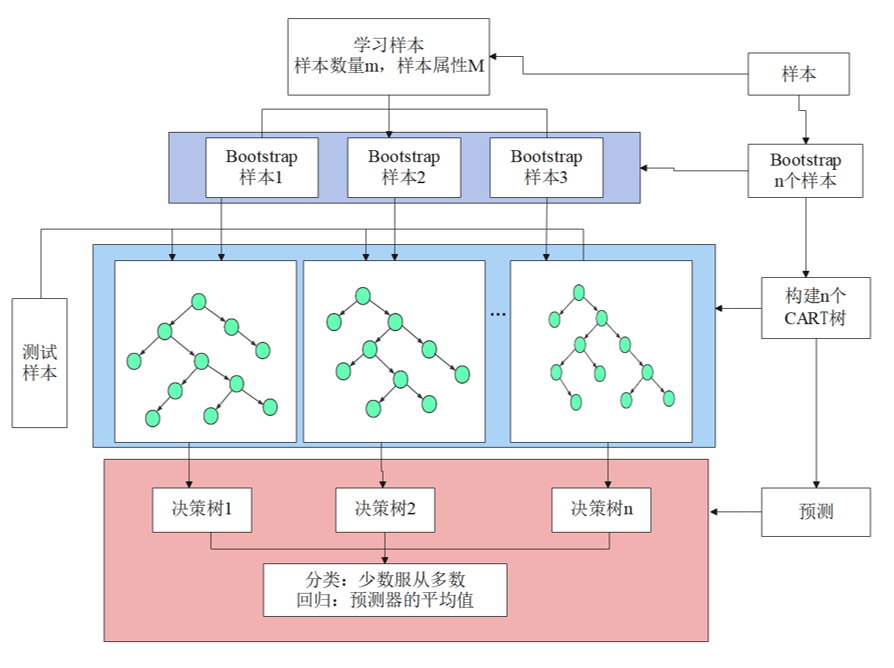
\includegraphics[width = \linewidth]{figures/随机森林模型原理图 .png}
    \caption{随机森林模型原理}
    \label{fig:随机森林原理}
\end{figure}

假设 X与 Y 分别为随机森林模型的输入和输出变量,其中Y为连续变量,给定训练数据集:
\begin{equation}
\begin{aligned}
D=\left\{\left(x_1, y_1\right),\left(x_2, y_2\right), \cdots,\left(x_N, y_N\right)\right\}
\end{aligned}
\label{equ:9}
\end{equation}

可以通过遍历训练集数据的每个特征变量及其对应的特征值,将其定义为不同的区域。假设正在进行区域划分的切分变量为第i个变量,对应切分特征值为j,则:
\begin{equation}
\begin{aligned}
\left\{\begin{array}{l}
a_1(i, j)=\left\{x \mid x^i \leq j\right\} \\
a_2(i, j)=\left\{x \mid x^i>j\right\}
\end{array}\right.
\end{aligned}
\label{equ:10}
\end{equation}

通过不断的遍历划分,输入数据及被划分为L个子空间$a_1, a_2, \cdots, a_L$,且每一个子空间$a_1$都包含其对应的样本数据和输出值$\beta_1$,则此时模型的解为:
\begin{equation}
\begin{aligned}
f(x)=\sum_{l=1}^L \beta_l I \quad\left(x \in \alpha_l\right)
\end{aligned}
\label{equ:11}
\end{equation}

采用和方差度量,度量目标是对于划分特征i,对应划分点j两边的数据集D1和D2。使D1和D2各自集合的均方差最小,同时D1和D2的均方差之和最小。其表达式为:
\begin{equation}
\begin{aligned}
\left.{\underset{i, j}{\min }[}_{\beta_1}^{\min } \sum_{x_i \in \alpha_1(i, j)}\left(y_l-\beta_1\right)^2+\sum_{\beta_2}^{\min } \sum_{x_l \in \alpha_2(i, j)}\left(y_l-\beta_2\right)^2\right]
\end{aligned}
\label{equ:12}
\end{equation}
\subsubsection{模型建立与求解}
{\textbf{初步建模}}\par
对于血肿扩张判定模型来说,其输入变量$X$为表1中患者的个人史,疾病史,发病相关(字段E至W)、“表2”中其影像检查结果(字段C至X)及“表 3”其影像检查结果(字段C至AG)等信息;输出变量$Y$为病人发生血肿扩张事件的概率。由于题目中并没有限定只对病人的血肿疾病信息进行判定分析,因此,我们模型的输入变量除去病人的血肿疾病信息,还包含了病人的水肿疾病信息。

考虑到第一问结果中,发生48小时内血肿扩张事件的病人仅有23名,仅占被研究患者总数的23\%。这种不平衡的数据可能导致模型为了追求精度,将占比少的数据信息权重调低,使得模型脱离了现实意义。因此,我们选择对血肿扩张患者的信息进行重采样,并对其各信息均加入白噪声,以提高模型的鲁棒性,降低数据的不平衡性。

根据输入变量的连续性、离散型以及类别性质,首先对输入变量进行初步处理,将输入变量转译为85个float型变量、8个int型变量和15个bool型变量。然后,通过粒子群算法优化LightGBM和随机森林模型的超参数,确定二者的超参数如表\ref{tab:2}所示。

\begin{table}[ht]
\centering
\caption{LightGBM\&随机森林超参数设置}
\label{tab:2}
\fontsize{11}{9}\selectfont
\renewcommand\tabcolsep{6pt}
{
\begin{tabular}{cc|cc}
\toprule[1.2pt]
\multicolumn{2}{c|}{\textbf{LightGBM}} & \multicolumn{2}{c}{\textbf{随机森林}} \\ \midrule
学习率                & 0.03          & 树的数量           & 300     \\
叶子节点数              & 128           & 最大叶子节点数        & 15000   \\
特征抽样比例             & 0.9           & 随机种子           & 0       \\
叶子节点最小数据量          & 5             & Bootstrap抽样    & TRUE    \\  \bottomrule[1.2pt]
\end{tabular}}
\end{table}

训练模型,得到LightGBM和随机森林模型对患者发生血肿扩张概率的预测准确率分别达到了96.6667\%和 96.6666667\%,具体训练结果如表\ref{tab:3}所示。\\
\begin{table}[ht]
\centering
\caption{LightGBM \& 随机森林结果展示}
\label{tab:3}
\fontsize{11}{9}\selectfont
\renewcommand\tabcolsep{6pt}
{
\begin{tabular}{ccc}
\toprule[1.2pt]
\textbf{模型}                        & LightGBM & 随机森林 \\ \hline
\textbf{score\_val}                & 0.966667      & 0.966666667      \\
\textbf{pred\_time\_val}           & 0.000998      & 0.025336027      \\
\textbf{fit\_time}                 & 0.228427      & 0.30355835       \\
\textbf{pred\_time\_val\_marginal} & 0.000998      & 0.025336027      \\
\textbf{fit\_time\_marginal}       & 0.228427      & 0.30355835       \\
\textbf{stack\_level}              & 1             & 1                \\
\textbf{can\_infer}                & TRUE          & TRUE             \\
\textbf{fit\_order}                & 13            & 5                \\  \bottomrule[1.2pt]
\end{tabular}}
\end{table}

{\textbf{Nelder-Mead \& 集成学习调优}}\par
为了进一步提高模型对血肿扩张概率预测的准确度,我们决定使用Nelder-Mead和集成学习结合的方法,对两模型进一步调优并加权集成。

Nelder-Mead是一种用于单目标优化的迭代数值优化算法,通常用于寻找函数的最小值。其主要原理是主要原理是通过不断寻找单个函数的最优参数值,以使该函数的输出值最小化或最大化。

集成学习是将多个不同的机器学习模型结合在一起,以提高预测的准确性和鲁棒性的策略。通过采用不同的算法和数据特征,集成模型可以降低过拟合风险,提高模型的泛化能力,并通过投票策略获得更可靠的预测结果。这种方法能够最大程度地利用各个模型的优势,使整体模型更强大。

对LightGBM和随机森林做集成学习的具体流程如图\ref{fig:集成流程图}所示。
\begin{figure}[h]
    \centering
    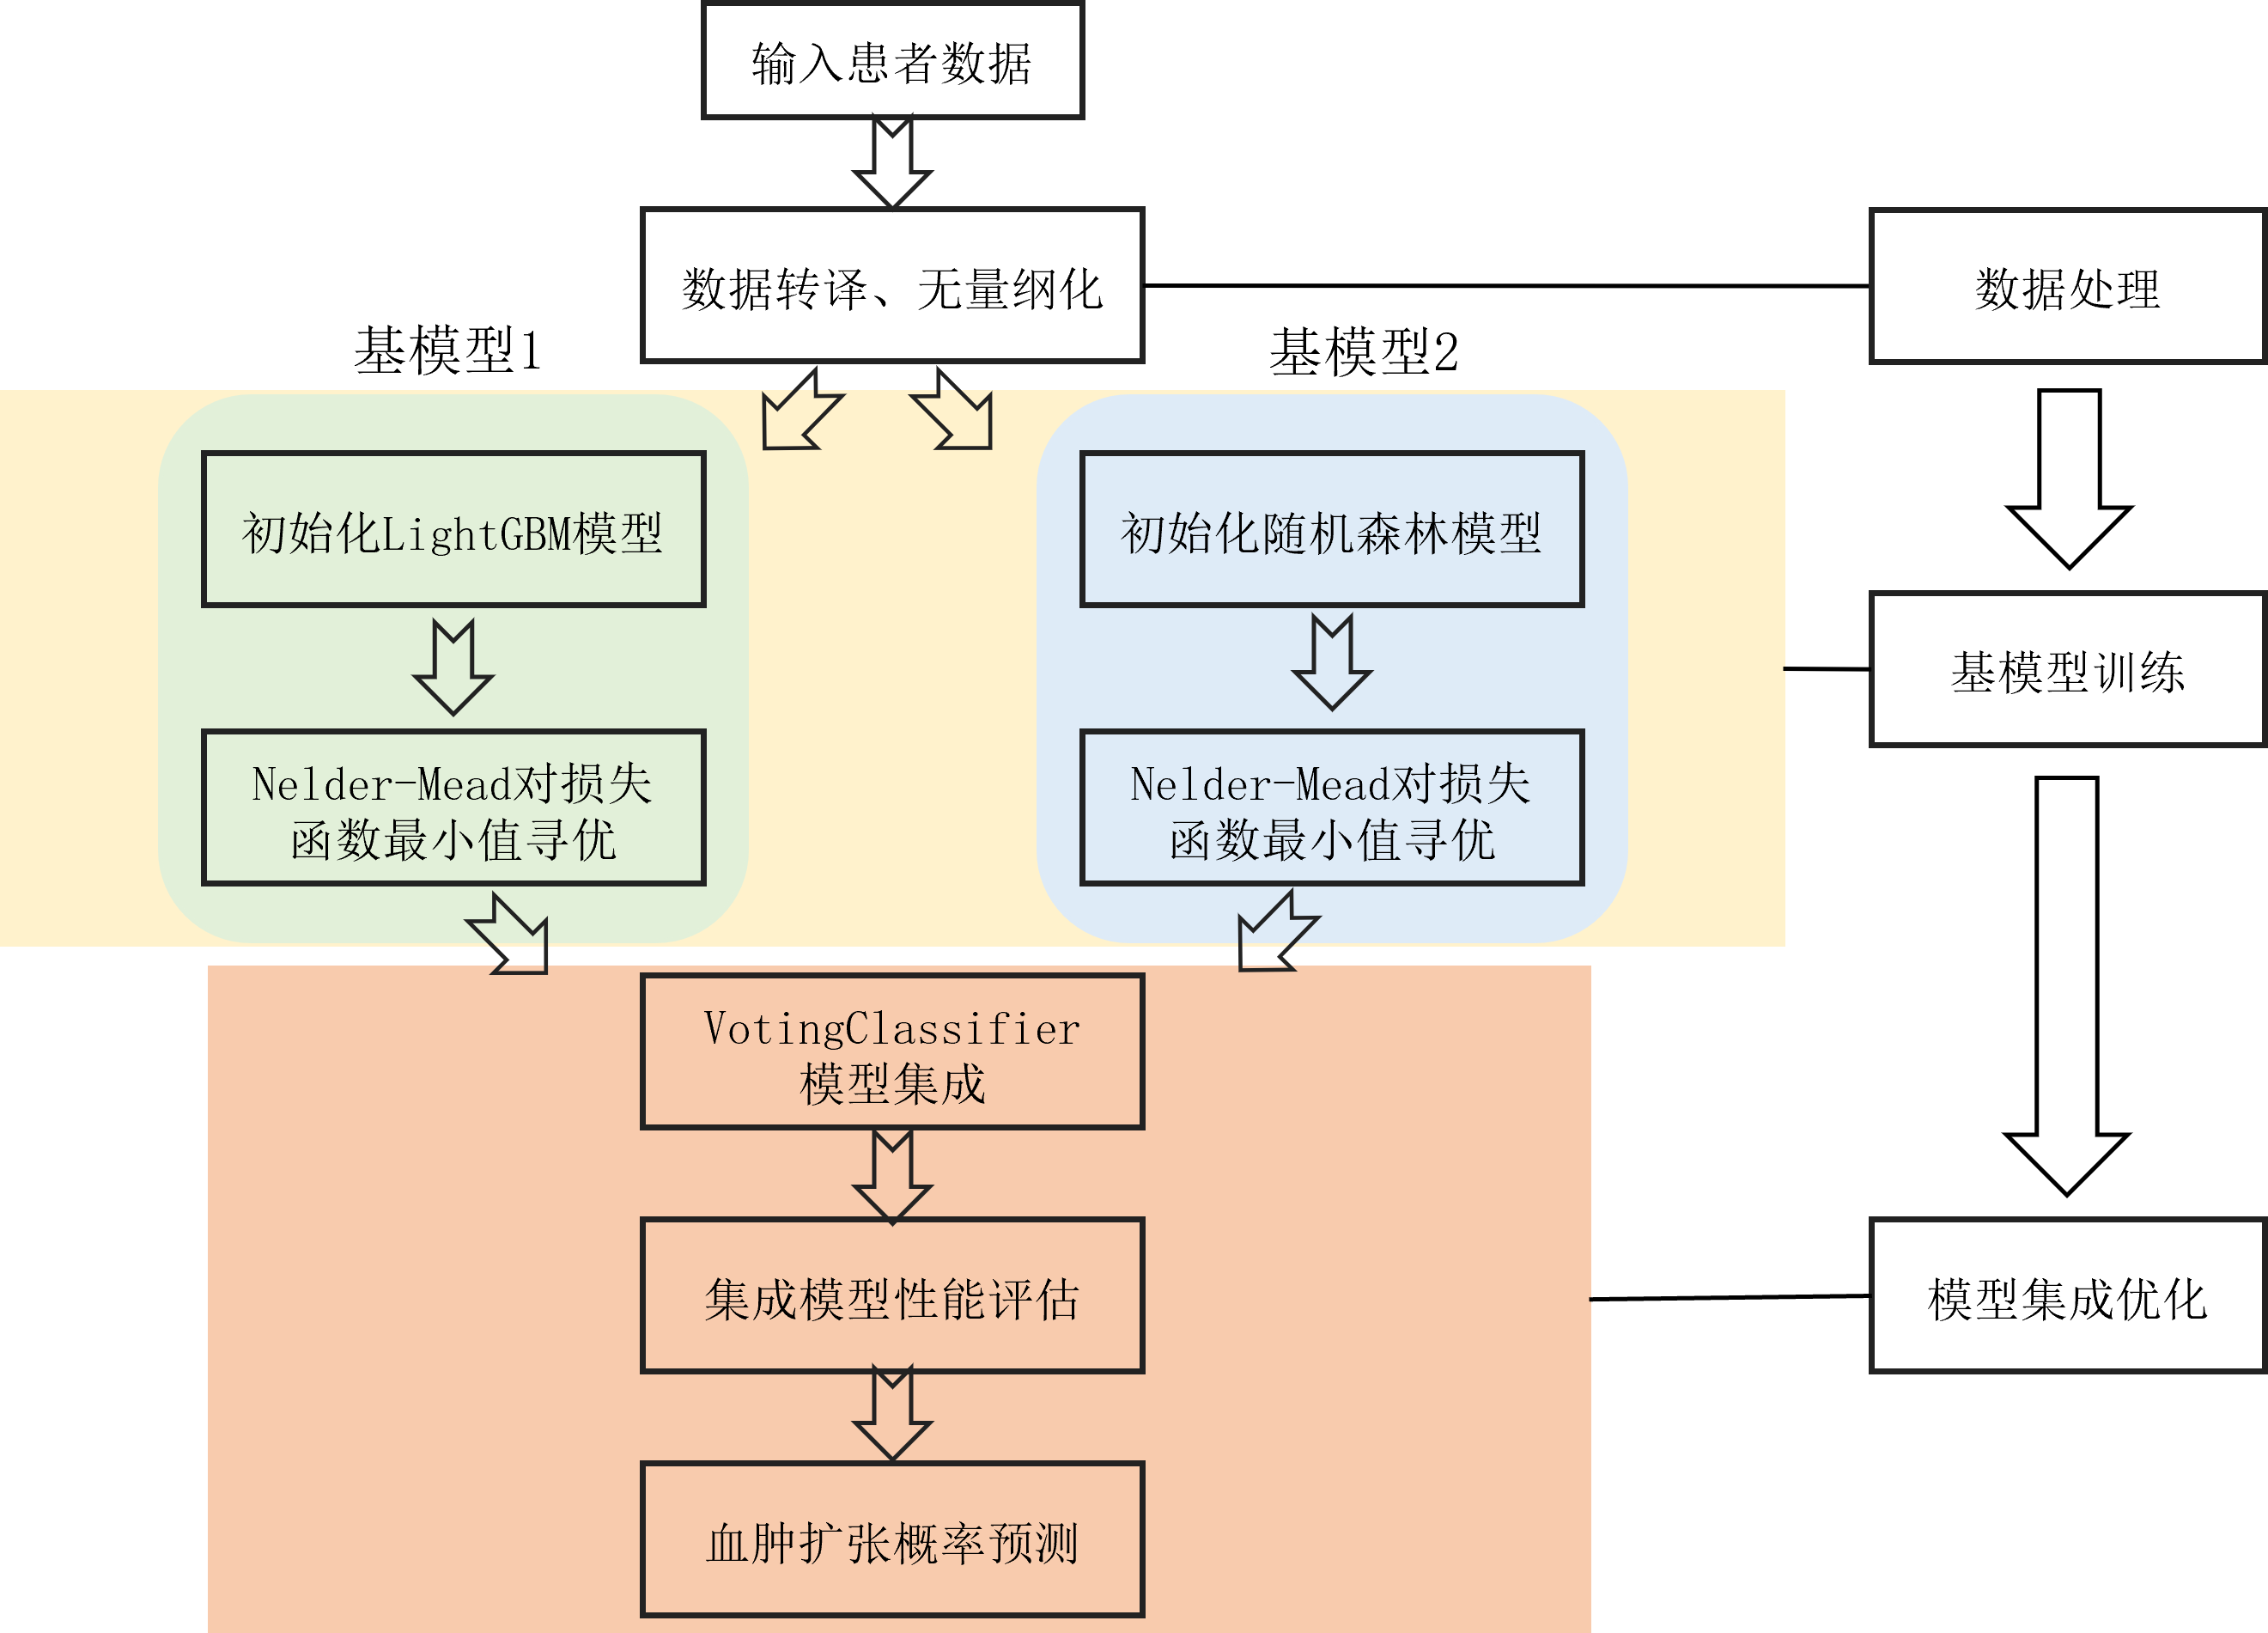
\includegraphics[width = \linewidth]{figures/集成原理.png}
    \caption{集成流程}
    \label{fig:集成流程图}
\end{figure}

为了实现对LightGBM和随机森林的进一步调优和集成,首先将Nelder-Mead的目标函数$target$设置为LightGBM和随机森林的损失函数$l$,并对其做最小值寻优。然后使用VotingClassifier集成学习器对二者进行权重分配并整合拟合结果。最后,使用优化好的LightGBM和随机森林对患者发生血肿扩张事件的概率再一次进行预测,并使用VotingClassifier确立的权重对结果进行加权求和。经检验,集成后的模型对患者发生血肿扩张事件概率的预测精度达到了99\%,相较集成之前,误差下降了70\%。这为我们更准确地识别潜在高风险患者,采取及时的干预措施,提供了有力的保障。


\section{问题二建模与求解}
\subsection{问题分析}
为了研究血肿周围水肿的发生及进展,并探索治疗干预和水肿进展的关联关系。在这一环节中,我们将建立新的、更加高效的模型,为血肿、水肿患者的临床治疗提供可信的信息预测。

在本问中,我们一共要完成四项任务:
\begin{enumerate}
    \item 根据“表2”前100个患者的水肿体积和重复检查时间点,建立适当的数学模型,从而构建全体患者水肿体积随时间进展曲线,并计算前100个患者的真实值和所拟合曲线之间的残差;
    \item 将患者根据某些特征(例如,性别、年龄、疾病类型等)分为不同的亚组。然后,针对每个亚组构建不同人群的水肿体积随时间进展曲线,并计算前100个患者的真实值和曲线之间的残差;
    \item 建立合适的数学模型,剖析不同治疗方法对水肿体积进展模式的影响;
    \item 构建血肿体积、水肿体积和治疗方法之间的散点图或其他合适的可视化模型,分析血肿体积、水肿体积及治疗方法三者之间的关系。
\end{enumerate}
    

\subsection{第一问模型的建立与求解}
针对第一问,我们需要根据“表2”中的数据,构建一个水肿体积随时间进展的曲线,研究患者水肿体积的大小与发病时间的关系,并计算前100个患者水肿体积真实值和所拟合曲线之间存在的残差。具体来说,我们可以使用曲线拟合的方法,来计算真实值和所拟合曲线之间的残差,本文选用混合线性预测和BiLSTM相结合的方法,对患者水肿体积大小随时间的发展情况进行拟合。
\subsubsection{混合线性预测模型}
混合线性模型(Mixed Linear Model)是一种常用的统计学模型\cite{zhang2010mixed},用于分析多个因素对某个因变量的影响。其中,混合线性模型结合了线性模型和随机效应模型,可以同时考虑固定效应和随机效应的影响。

在混合线性模型中,我们假设存在一个固定效应和一个随机效应。固定效应表示某个因素对因变量的影响,而随机效应表示个体之间的差异。因此,混合线性模型可以同时考虑这些因素的影响,并且通过线性模型来拟合这些效应。

具体来说,混合线性模型的公式如下:
\begin{equation}
\begin{aligned}
y=X \beta+z \gamma+e
\end{aligned}
\label{equ:12}
\end{equation}

其中,$y$是因变量,$X$是固定效应的系数矩阵,$\beta$是固定效应的系数向量,
$z$是随机效应的系数矩阵,$\gamma$是随机效应的系数向量,$e$是误差项。

混合线性模型中的随机效应可以表示为:
\begin{equation}
\begin{aligned}
z=Z \theta+R(u)
\end{aligned}
\label{equ:13}
\end{equation}

其中,$Z$是随机效应的系数矩阵,$\theta$是随机效应的系数向量,$R(u)$是一个随机过程,表示个体之间的差异。因此,混合线性模型的完整公式如下:
\begin{equation}
\begin{aligned}
y=X \beta+z \gamma+e=X \beta+Z \theta+R(u)+e
\end{aligned}
\label{equ:14}
\end{equation}

其中,$X \beta$是固定效应的影响,$Z \theta$是随机效应的影响,$R(u)$是随机误差项的影响。

\subsubsection{BiLSTM模型}
BiLSTM(Bidirectional LSTM)是一种循环神经网络(RNN)模型,它结合了前向和后向的LSTM单元,能够处理序列数据\cite{siami2019performance}。BiLSTM由两个LSTM单元组成,一个用于正向传播,另一个用于反向传播,从而能够更好地捕捉序列数据中的信息。

LSTM的主要组成结构为输入门$i_t$、遗忘门$f_t$和输出门$o_t$,同时在门结构中以$C_t$表示细胞单元的当前状态,$h_t$表示隐藏层状态,$x_t$为输入数据\cite{yu2019review}。先在输入层中,定义原始故障时间序列为$F_0=\left\{f_1, f_2, \cdots, f_n\right\}$,则划分的训练集和测试集可以表示为$F_{\text {tr }}=\left\{f_1, f_2, \cdots, f_m\right\}$和$F_{\text {te }}=\left\{f_m+1, f_m+2, \cdots, f_n\right\}$,满足约束条件$m<n$ 和 $m, n \in N$。然后对训练集中的元素$f_t$进行标准化,标准化后的训练集为$F^{\prime}{ }_{\mathrm{tr}}=\left\{f^{\prime}{ }_1, f^{\prime}{ }_2, \cdots, f^{\prime}{ }_m\right\}$。

为了适应隐藏层输入的特点,应用数据分割的方法对$F^{\prime}{ }_{\mathrm{tr}}$进行处理,设定分割窗口长度取值为$L$,则分割后的模型输入为$\mathrm{X}=\left\{X_1, X_2, \cdots, X_L\right\}$。则对应的理论输出为$\mathrm{Y}=\left\{Y_1, Y_2, \cdots, Y_L\right\}$。将$X$输入隐藏层,其包含$L$个按前后时刻连接的同构LSTM细胞。设定细胞状态向量大小为$S_{\text {state }}$,则$C_{P-1}$ 和 $H_{p-1}$两个向量的大小均为$S_{\text {state }}$。应用训练好的LSTM网络(表示为 $L S T M_{n e t}^*$ )进行预测。预测过程采用迭代的方法。首先理论输出$Y$的最后一行数据为$F_f=\left\{f^{\prime} m-L+1, f^{\prime} m-L+2, \cdots, f^{\prime} m\right\}$, 将 $F_f$ 输入 $L S T M_{n e t}^*$输出结果,然后将$Y_f$的最后$L-1$个数据点和$P_{\text {m+1 }}$合并为新的一行数据:
\begin{equation}
\begin{aligned}
Y_{f+1}=\left\{f^{\prime} m-L+2, f^{\prime} m-L+3, \cdots, f^{\prime} m\right\}
\end{aligned}
\label{equ:15}
\end{equation}

将 $Y_{f+1}$ 输入 $L S T M_{n e t}^*$ 则 $\mathrm{m}+2$ 时刻的预测值为 $P_{m+2}$。依次类推,得到的预测序列为$P_0=\left\{P_{m+1}, P_{m+2}, \cdots, P_n\right\}$ 接下来对 $P_0$ 进行 $z-$ score 反标准化(表示为 $de\_zscore$),得到最终的与测试集$F_{\text {te }}$对应的预测序列为$P_{t e}=d e \_z \operatorname{corere}\left(P_0\right)=\left\{P_{m+1}^*, P_{m+2}, \cdots P_n^*\right\}$,其中:
\begin{equation}
\begin{aligned}
p_k^*=p_k \sqrt{\sum_{t=1}^n\left(f_t-\sum_{t=1}^n f_t / n\right)^2 / n}+\sum_{t=1}^n f_t / n \quad m+1 \leq k \leq n, k \in N
\end{aligned}
\label{equ:16}
\end{equation}

类似地,将X的每行作为模型输入可以得到与训练集$F_{\text {tr }}$对应的拟合序列$P_{\text {tr }}$,最后通过计算$F_{\text {tr }}$和$P_{\text {tr }}$以及$F_{\text {te }}$和$P_{\text {te }}$的偏差定量地给出模型的拟合和预测精度。

在BiLSTM中,输入序列首先通过一个LSTM单元进行前向传播,然后将输出通过另一个LSTM单元进行反向传播。这个过程在每个时间步重复,直到达到序列的末尾。

BiLSTM的公式如下:
\begin{equation}
\begin{aligned}
h_t=f_1\left(h_{t-1}, x_t\right)
\end{aligned}
\label{equ:17}
\end{equation}

\begin{equation}
\begin{aligned}
h_t=g_1\left(h_{t-1}, x_t\right)
\end{aligned}
\label{equ:18}
\end{equation}

其中, $h_t$ 是当前时间步的输出, $h_{t-1}$ 是前一个时间步的输出, $x_t$ 是当前时间步的输入。 $f_1$ 和 $g_1$ 是LSTM单元的激活函数,用于计算当前时间步的输出。

BiLSTM模型的原理如图\ref{fig:BiLSTM原理}所示。
\begin{figure}[h]
    \centering
    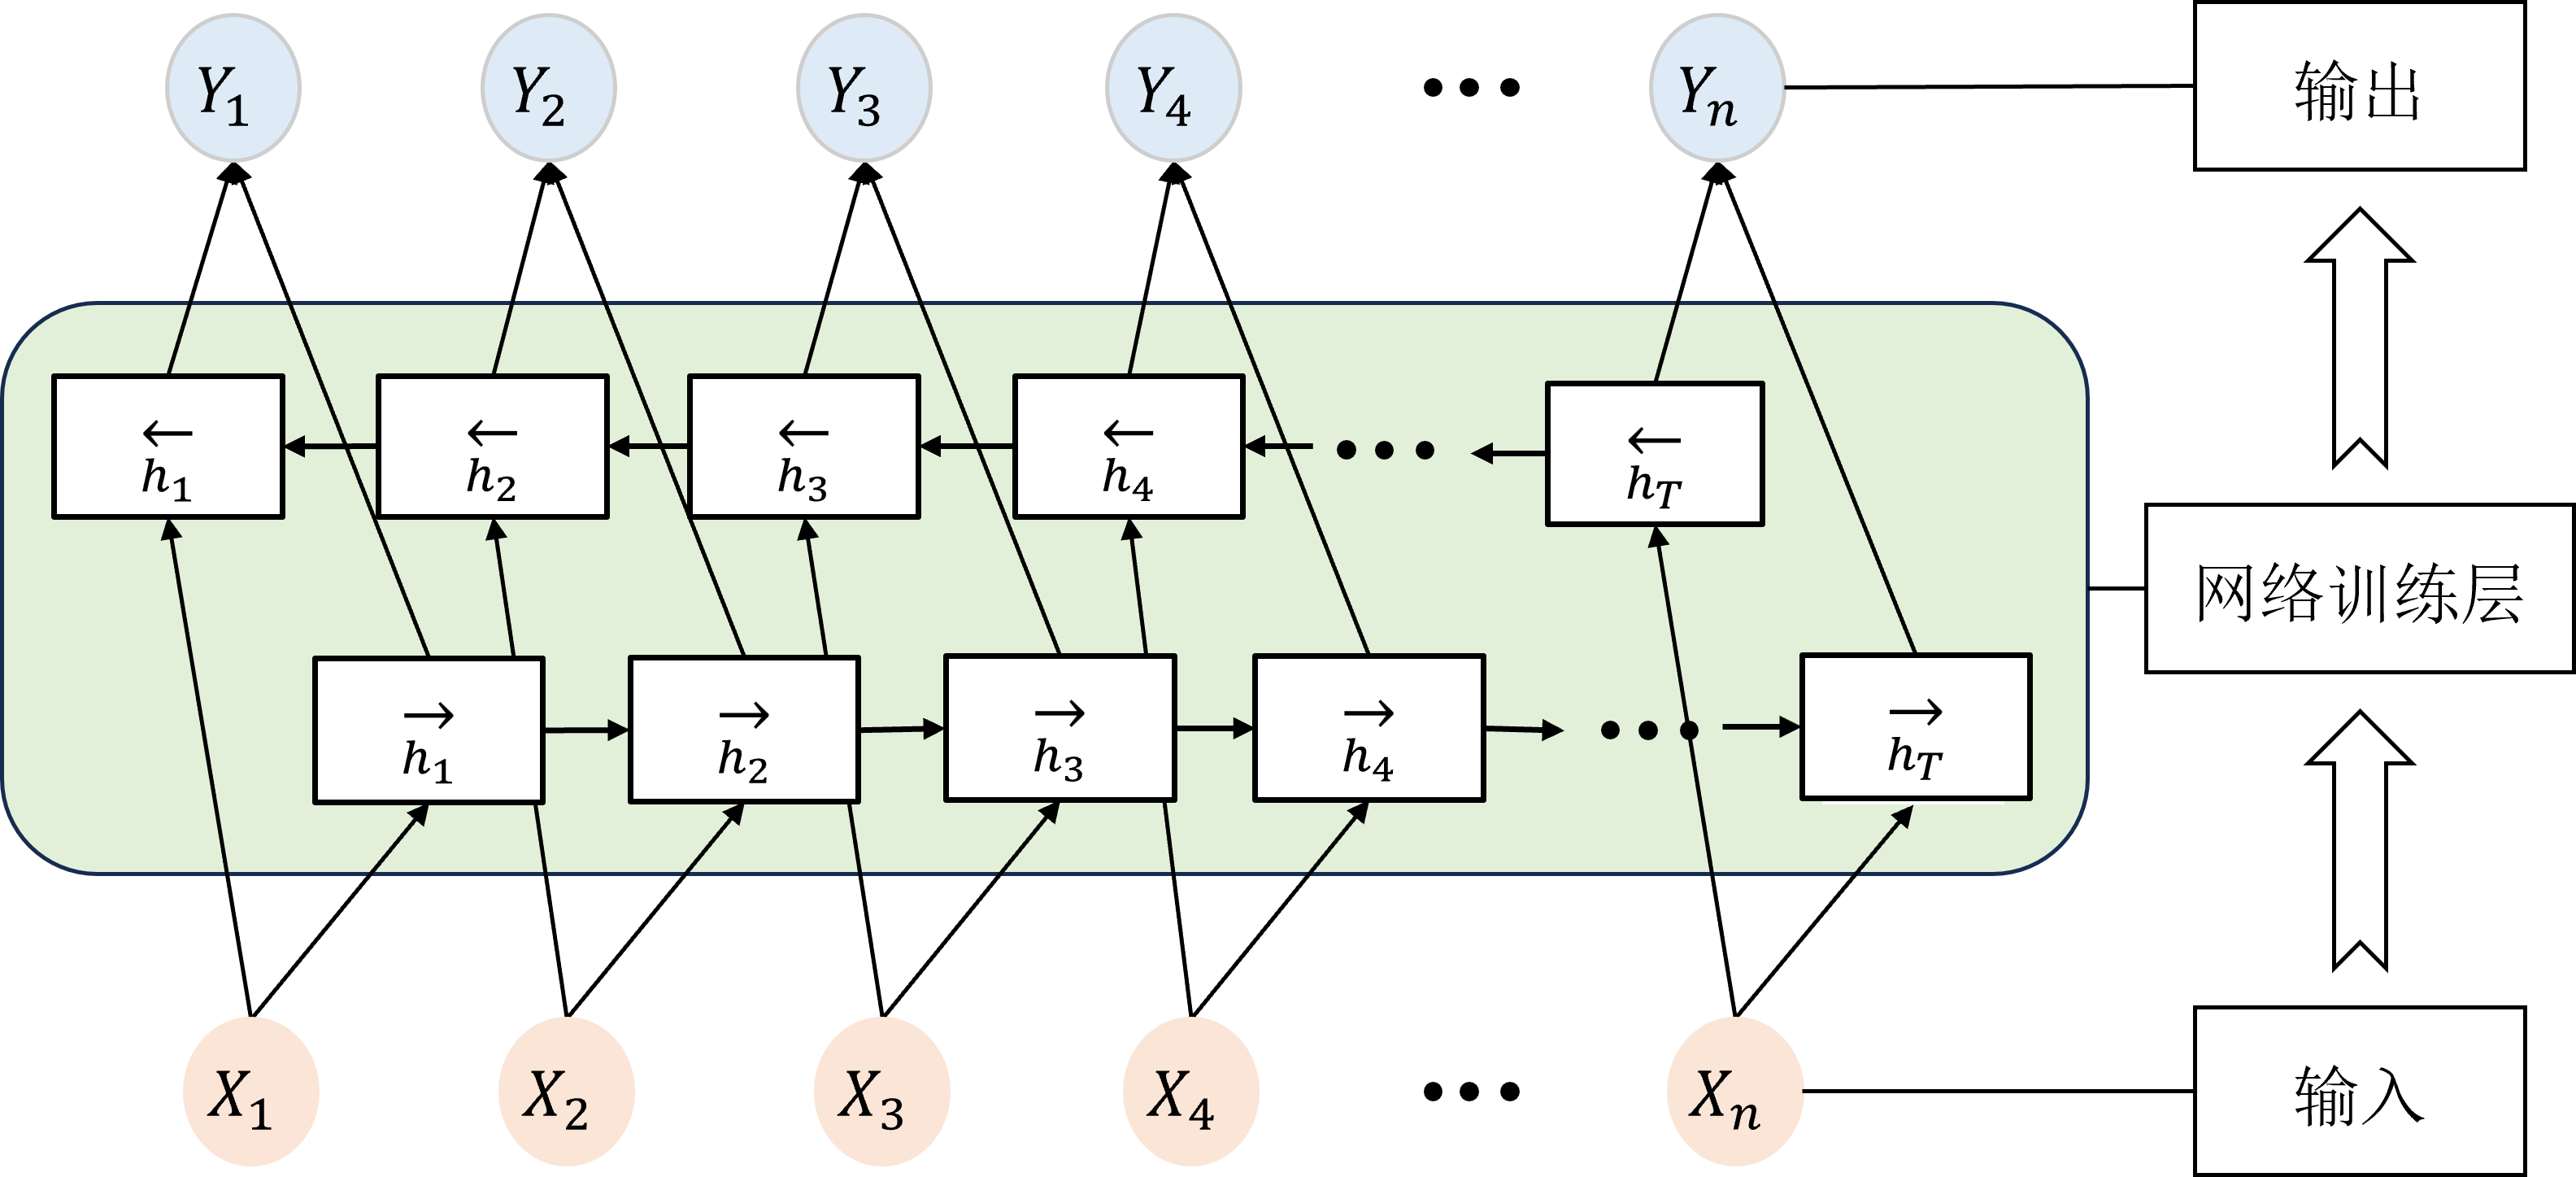
\includegraphics[width = \linewidth]{figures/BiLSTM原理图.png}
    \caption{BiLSTM原理}
    \label{fig:BiLSTM原理}
\end{figure}

\subsubsection{CEEMD模型}
CEEMD模型是一种用于分析非线性系统的方法\cite{yan2020novel},它可以分解出系统的各个模态,这也是混合线性预测模型和BiLSTM模型结合的基础。通过CEEMD模型,我们可以将原始数据分为分别适合与混合线性预测模型和BiLSTM模型的模态,并进行分别拟合,从而实现二者相结合的目的,提高模型的拟合精度。CEEMD的原理如图\ref{fig:CEEMD原理}所示。
\begin{figure}[h]
    \centering
    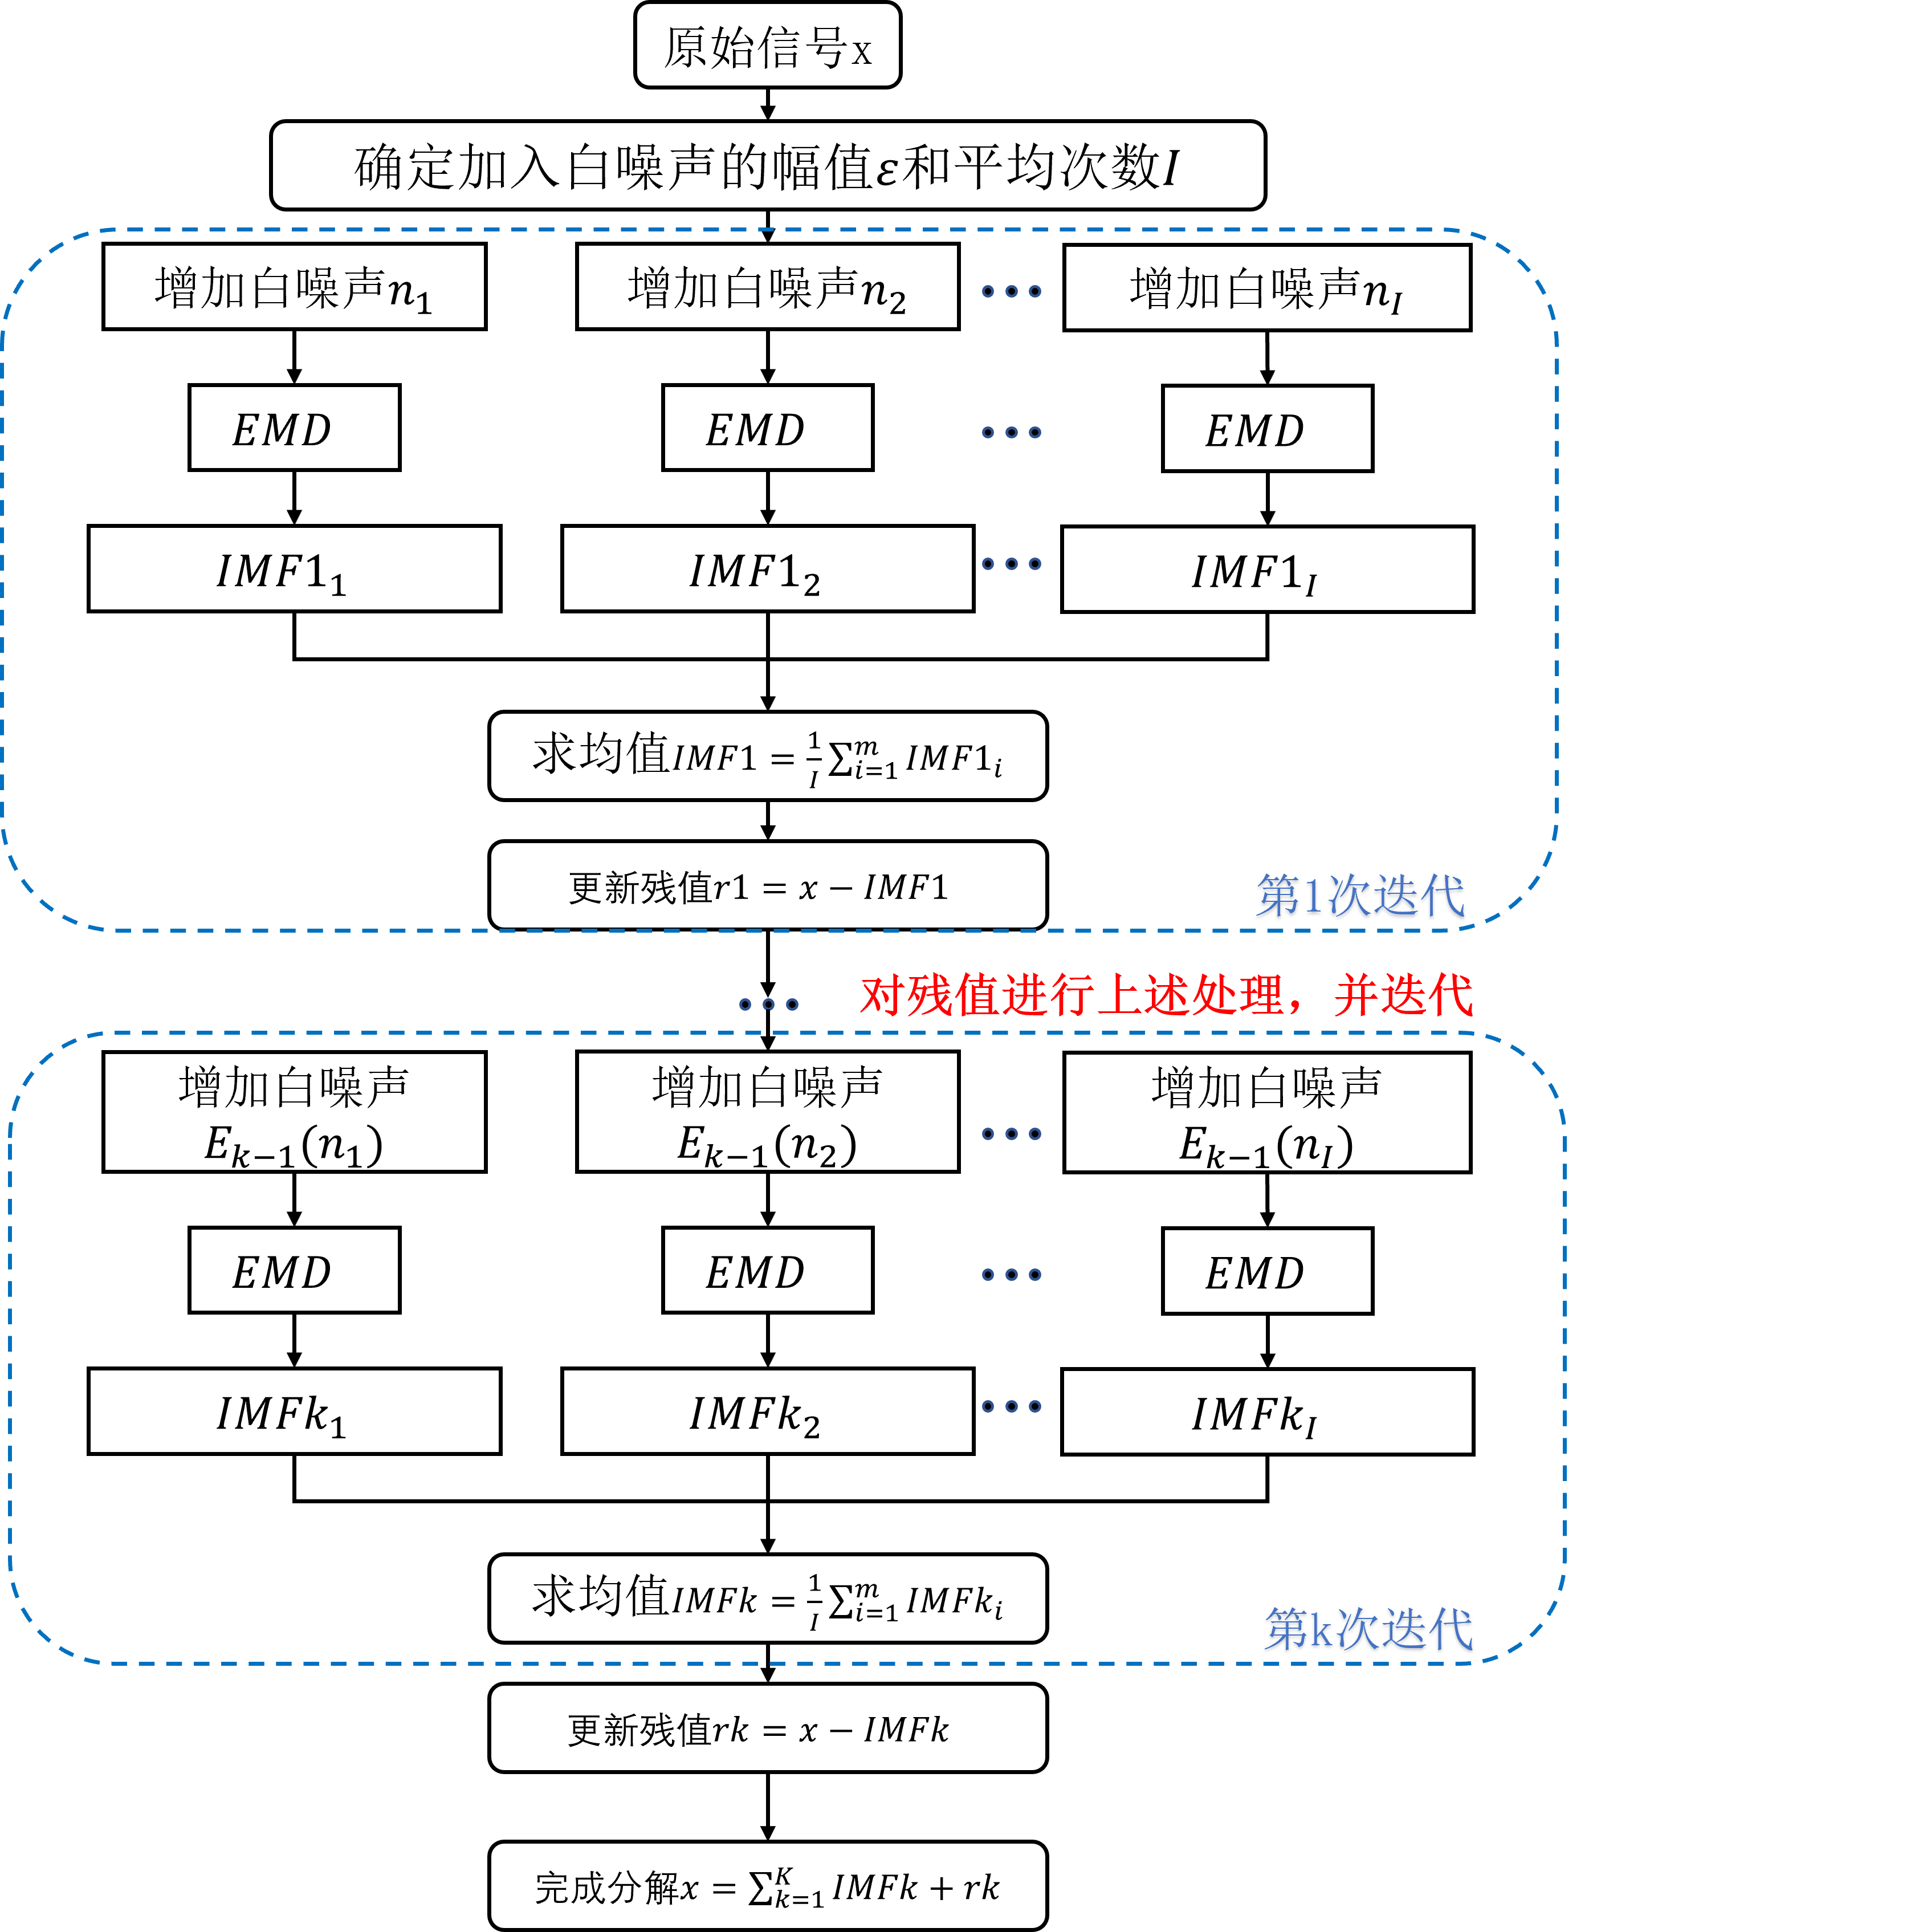
\includegraphics[width = \linewidth]{figures/CEEMD原理图.png}
    \caption{CEEMD原理}
    \label{fig:CEEMD原理}
\end{figure}


\subsubsection{模型参数的确立与求解}
为了研究全体患者水肿体积随时间进展的变化趋势,我们首先将前一百名患者的水肿体积信息以发病时间为初始节点,按照间隔时间进行排序。接着,将每名患者的水肿体积数据与发病时的初始体积作比值,得到每名患者水肿体积的相对大小随时间的变化表格。然后使用混合线性预测模型与BiLSTM模型结合的预测方式,对患者水肿体积和发病间隔时间进行拟合。拟合结果分为两块:对每名患者水肿体积初始大小的预测;对患者水肿体积的相对大小随时间变化的预测。

在确定模型的超参数之前,先对患者水肿体积大小和发病时间间隔的趋势进行初步分析,患者水肿体积大小随发病时间间隔的趋势如图\ref{fig:水肿体积大小趋势}示。
\begin{figure}[h]
    \centering
    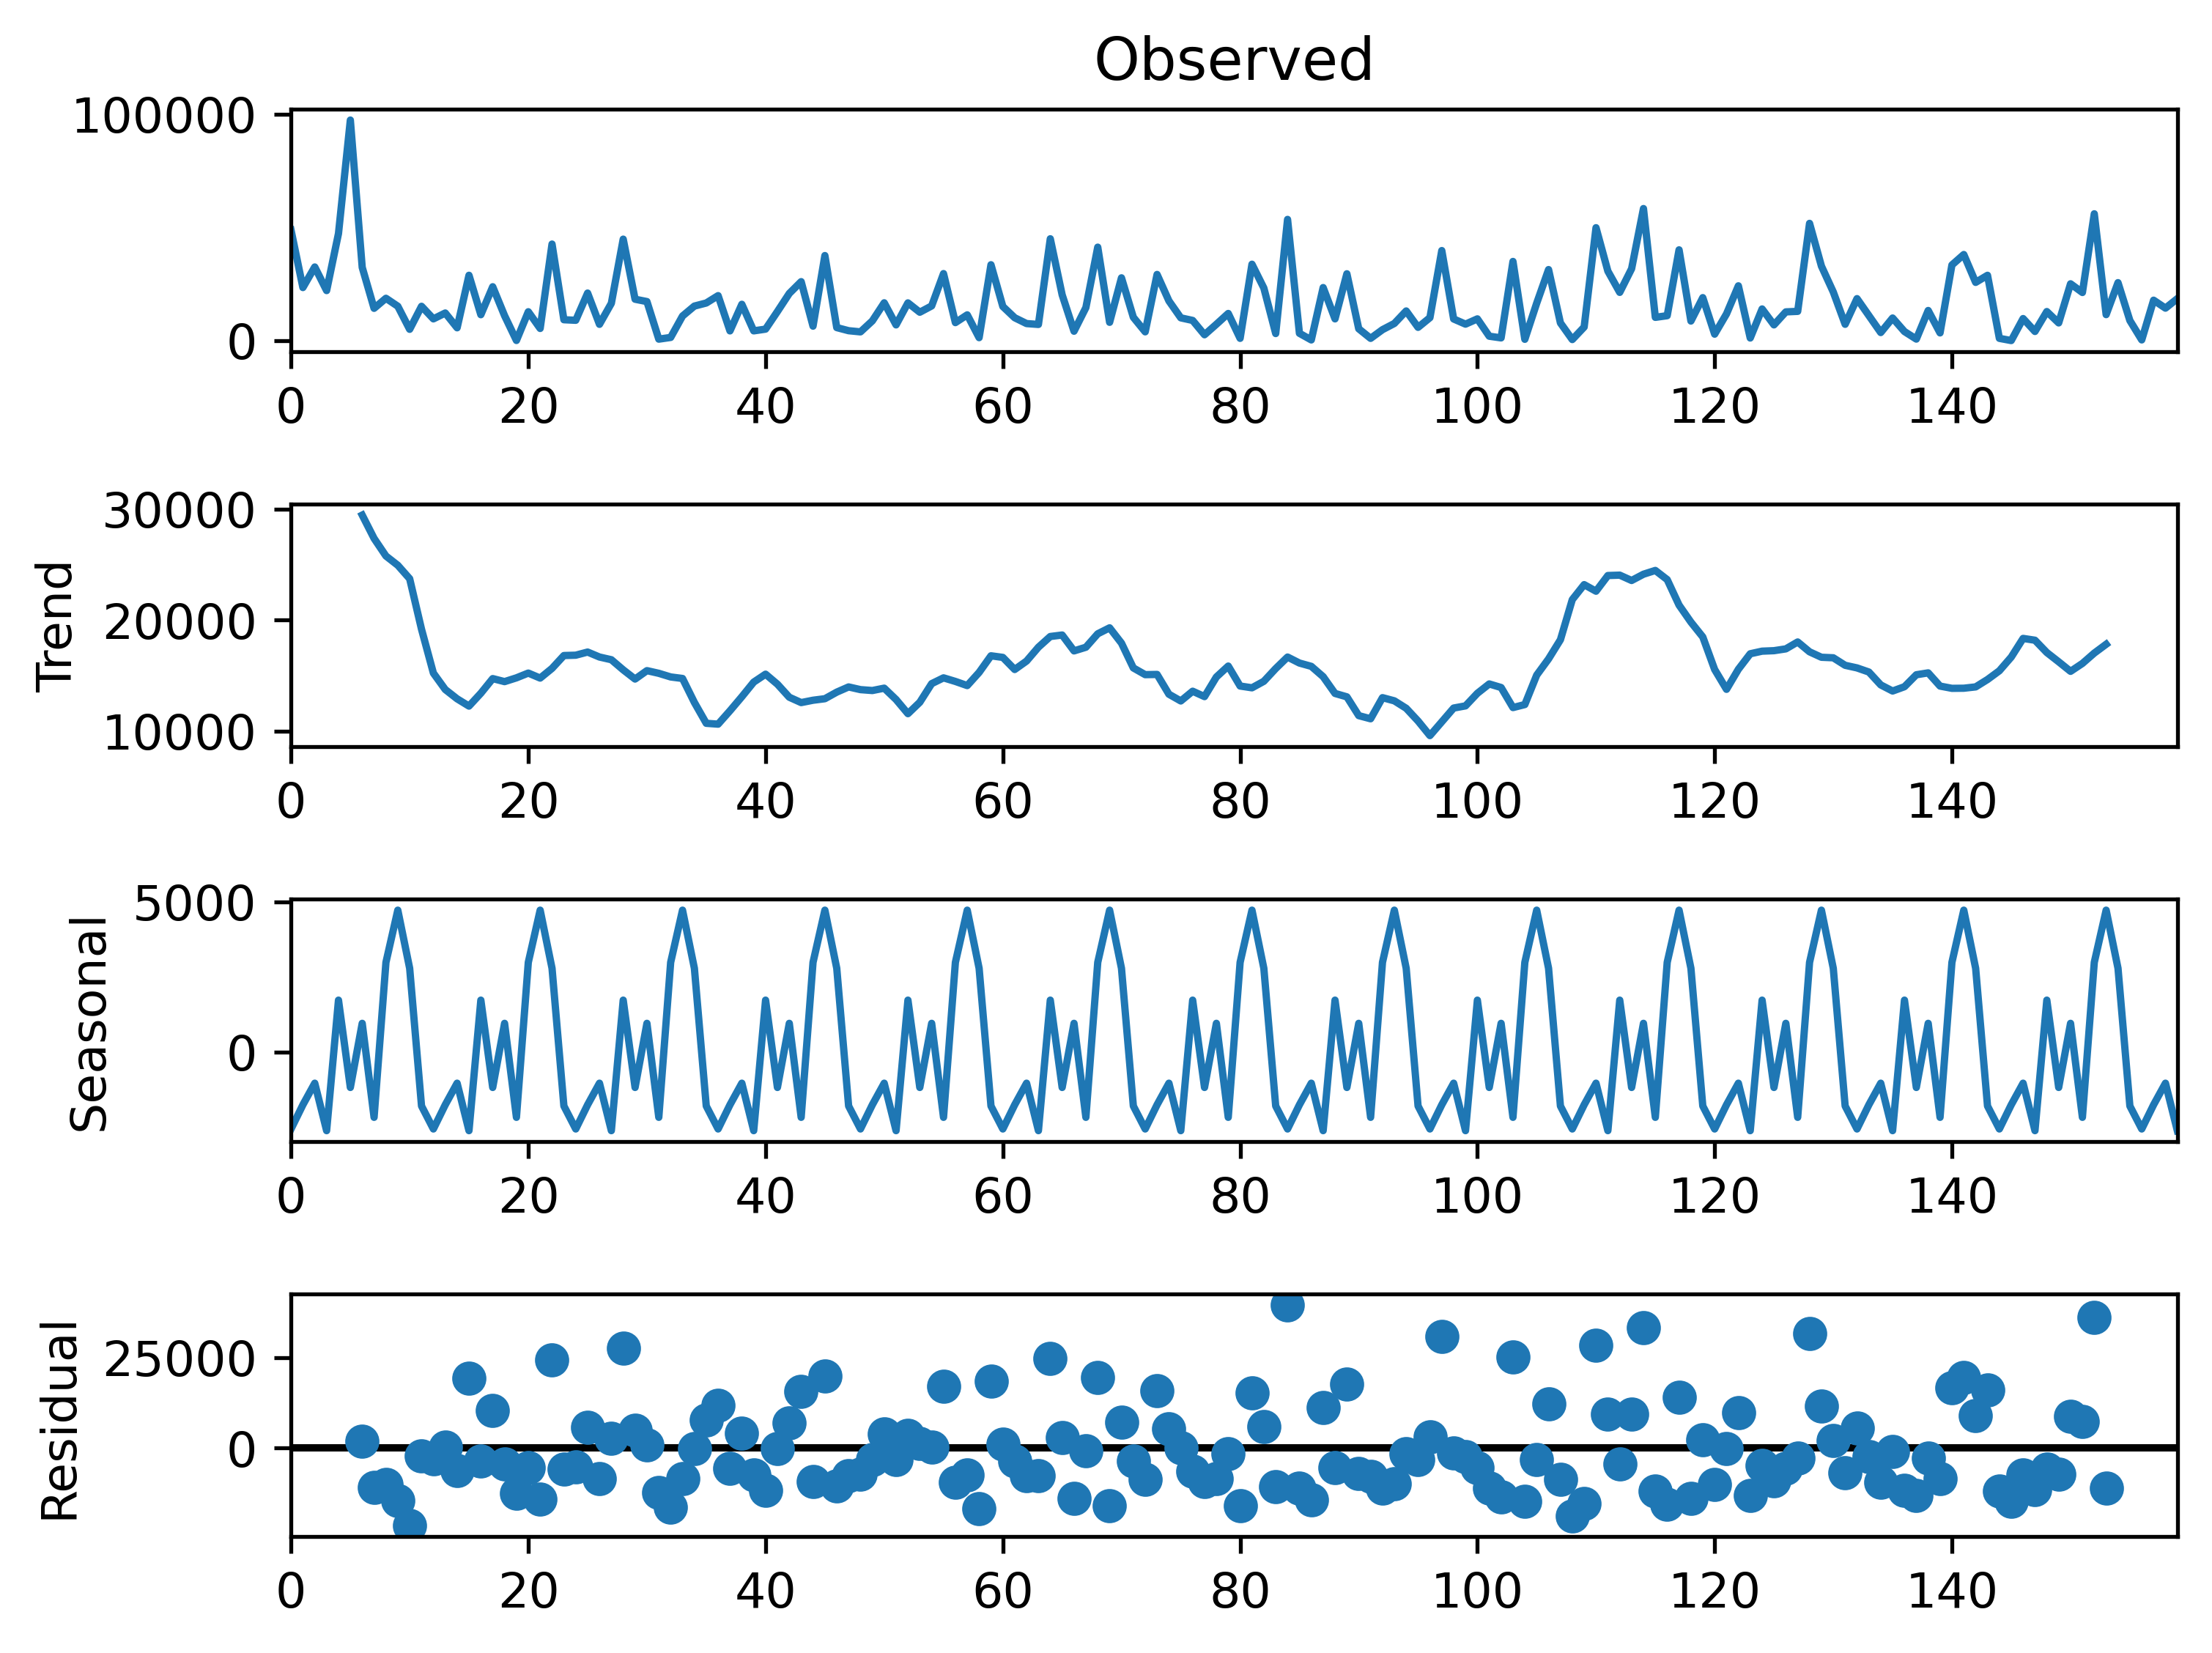
\includegraphics[width = \linewidth]{figures/seasonal_decompose.png}
    \caption{水肿体积大小随发病时间间隔的趋势}
    \label{fig:水肿体积大小趋势}
\end{figure}

除此之外,考虑到数据样本集合的大小,以及输出变量和输入变量的维度,我们需要选择合适的参数,用以优化模型的拟合效果。


{\bf 混合线性预测模型超参数确立:}对于此次任务,混合线性预测模型的主要超参数分别为intercept、time\_gap和Group Var。其中,intercept是常数项,用于平移模型输出的截距,为了对每名患者水肿体积的相对大小进行拟合,我们选用各患者水肿体积初始大小的平均值26020.755312作为intercept的取值;time\_gap表示时间间隔,用于控制时间序列模型的建模时间和步长,考虑到患者多次复查之间的时间间隔,以及模型的整体拟合效果,将该时间步长取值为-3.29294;Group Var表示组方差,用于体现不同组别之间的差异,从而对不同患者样本进行区分,避免模型过于拟合某一患者样本,对该超参数的值取0.648374。\par\par

{\bf BiLSTM模型超参数确立:}BiLSTM是由两个传播方向相反的LSTM模型组成的,因此只需确定LSTM模型的超参数即可。LSTM模型的结构示意如图\ref{fig:LSTM结构示意}所示。
\begin{figure}[h]
    \centering
    
\includegraphics[width = \linewidth]{figures/LSTM结构示意.png}
    \caption{LSTM结构示意图}
    \label{fig:LSTM结构示意}
\end{figure}

LSTM的主要模型超参数有num\_epochs、batch\_size、learning\_rate和dropout。
\begin{enumerate}
    \item num\_epochs指定模型训练的迭代次数,考虑到患者样本数据集并不大,不会对模型训练参生较大的负荷,因此为了提高模型的训练精度,我们将num\_epochs设置为100。
    \item batch\_size表示每次训练时使用的样本数量,当该参数较大时,模型的训练速度和收敛速度会提高,但是同样会造成计算成本的上升,考虑到二者的综合博弈,将batch\_size设置为32。
    \item learning\_rate为模型更新参数时的学习率,学习率越大,模型更新参数的速度越快,但可能会造成过拟合;学习率越小,模型更新参数的速度越慢,但可以减少过拟合的风险。为了防止过拟合,并尽可能的提高模型的训练精度,将learning\_rate设置为0.001。
    \item dropout为训练过程中丢弃神经元(即随机抑制神经元的活动)的概率。丢弃神经元可以防止过拟合,减少模型对训练数据的依赖性。为了控制模型的复杂度,提高模型的泛化能力,将dropout设置为0.5。
\end{enumerate}\par

{\bf 模型结果展示}\par
将患者样本的水肿体积数据以及发病间隔时间带入模型,并使用CEEMD模型对初始数据做模态分解,分解结果如图\ref{fig:模态分解结果}所示。
\begin{figure}[h]
    \centering
    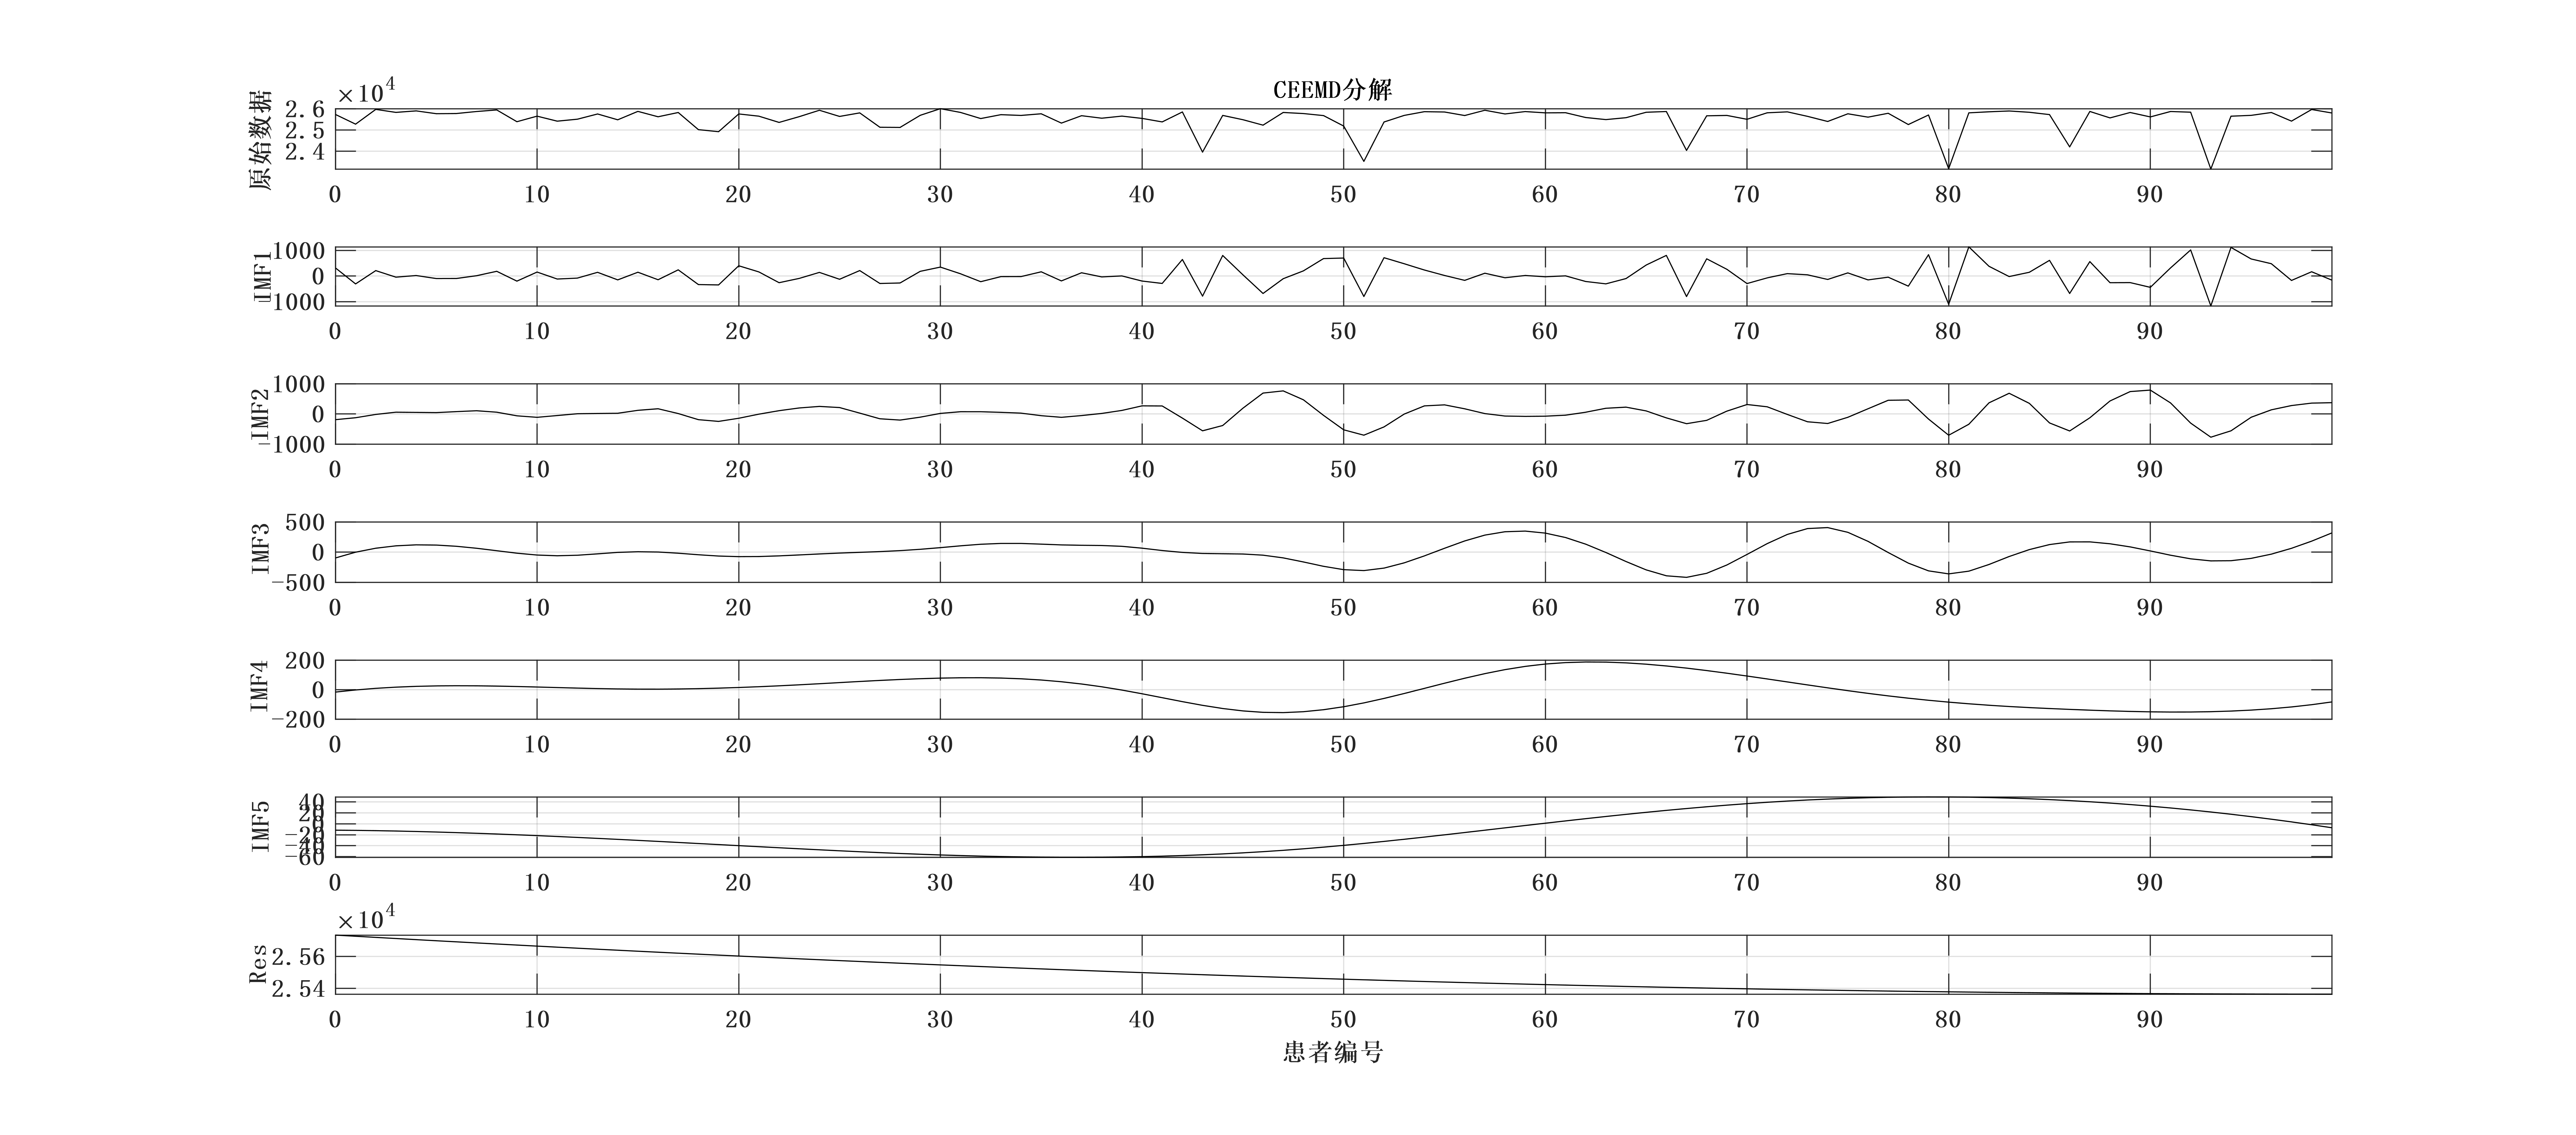
\includegraphics[width = \linewidth]{figures/模态分解结果.png}
    \caption{模态分解结果}
    \label{fig:模态分解结果}
\end{figure}

对两组不同模态的数据分别采用混合线性预测模型和BiLSTM模型进行拟合,然后对拟合结果进行加权求和,最后将同一患者样本的拟合误差取平均值,模型拟合效果如图\ref{fig:2a拟合效果}所示。
\begin{figure}[h]
    \centering
    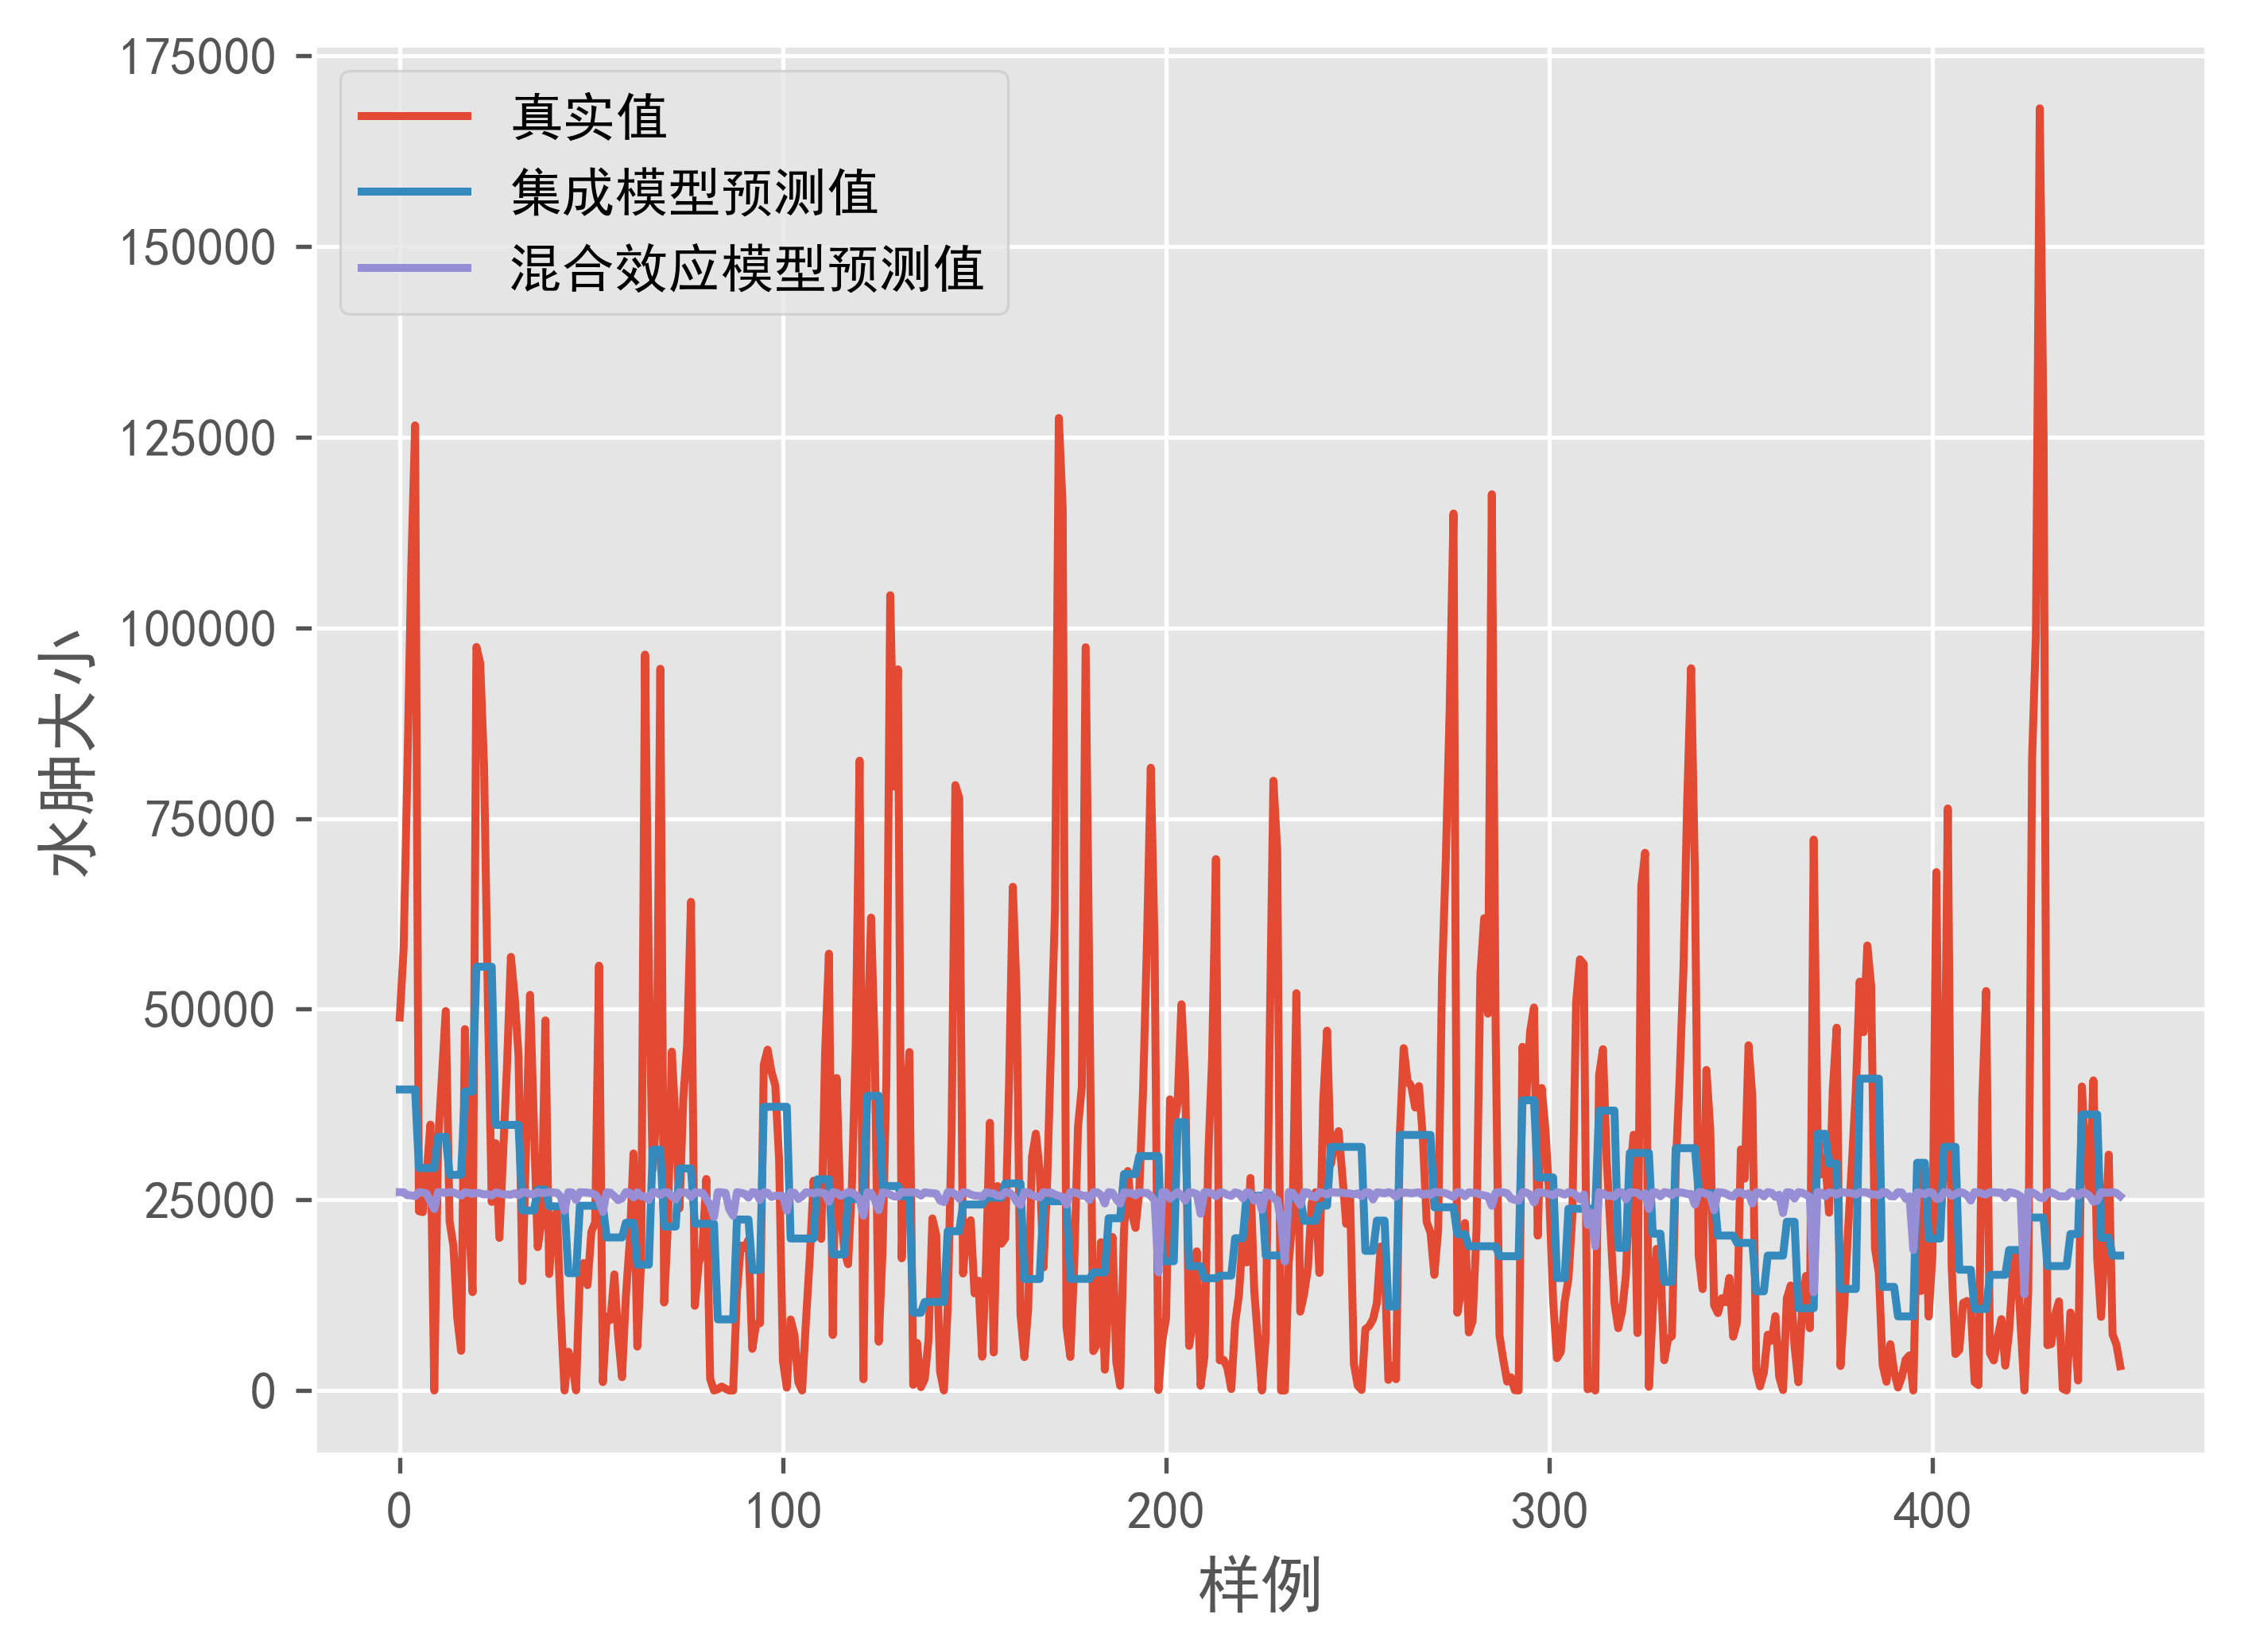
\includegraphics[width = \linewidth]{figures/p2a模型预测结果.png}
    \caption{模型拟合曲线}
    \label{fig:2a拟合效果}
\end{figure}


患者水肿体积大小随时间进展的拟合结果如表\ref{tab:4}所示。
\begin{table}[ht]
\centering
\caption{拟合结果展示}
\label{tab:4}
\fontsize{11}{9}\selectfont
\renewcommand\tabcolsep{6pt}
{
\begin{tabular}{cccc}
\toprule[1.2pt]
\textbf{患者ID}   & \textbf{水肿体积预测值} & \textbf{水肿体积实际值} & \textbf{预测误差} \\
\midrule
\textbf{sub001} & 39472.44922      & 84583            & -45110.55078  \\
\textbf{sub002} & 29165.27344      & 22039.8          & 7125.473438   \\
\textbf{sub003} & 33256.30859      & 41226.66667      & -7970.358073  \\
\textbf{sub004} & 28283.60742      & 13972.75         & 14310.85742   \\
\textbf{…}      & …                & …                & …             \\
\textbf{sub099} & 20033.80469      & 20034.33333      & -0.528645833  \\
\textbf{sub100} & 17693.62109      & 5530.333333      & 12163.28776   \\ \bottomrule[1.2pt]
\end{tabular}}
\end{table}

分析拟合结果可知,模型对患者水肿体积大小和发病时间间隔拟合曲线的RMSE为25670.456。这是因为,相同的时间间隔对应的患者样本个体不同,在这样但输入的限制下,输入数据的信息可能无法充分地传递给多个输出,导致输出结果的不准确。在对患者样本进行进一步聚类处理后,模型效果会有明显的提升。

\subsection{第二问模型的建立与求解}
为了研究患者水肿体积随时间进展模式的个体差异,并构建不同人群的水肿体积随时间进展曲线。我们首先需要对患者样本进行聚类,将其按照不同的特征化成3-5个亚组。然后,在使用调优后的混合预测模型对各自亚组下的患者样本水肿体积随时间的变化趋势做进一步拟合。
\subsubsection{K-means聚类}
K-means聚类是一种无监督学习算法,用于将数据集分为K个不同的簇\cite{likas2003global}。其基本思想是将数据集中的每个数据点分配到距离其最近的簇中心,然后不断迭代更新簇中心和数据点的簇分配,直到收敛。K-means聚类的具体流程如下所示:
\begin{enumerate}
    \item  首先,随机选择K个数据点作为初始的簇中心。
    \item  对于每个数据点,计算其到K个簇中心的距离,并将其分配到距离最近的簇中。
    \item  对于每个簇,重新计算其簇中心,即计算簇中所有数据点的均值。
    \item  重复步骤2和3,直到簇中心不再改变或达到最大迭代次数。
\end{enumerate}\par
在计算每个数据点到簇中心的距离时,可以采用欧几里得距离,其计算公式如下:
\begin{equation}
\begin{aligned}
D(i,j) = \sqrt{(x_{1j} - x_{1i})^{2} + (x_{2j} - x_{2i})^{2} + \cdots + (x_{nj} - x_{ni})^{2}}
\end{aligned}
\label{equ:欧几里得距离}
\end{equation}

其中,$D(i,j)$表示第$i$个点和第$j$个点之间的欧几里得距离,$x_{n i}$ 和 $x_{n j}$分别表示第$i$个点和第$j$个点的第$n$个坐标值。

\begin{table}[ht]
\centering
\caption{feature importance展示}
\label{tab:importance_b}
\fontsize{11}{9}\selectfont
\renewcommand\tabcolsep{6pt}
{
\begin{tabular}{cc}
\toprule[1.2pt]
\textbf{特征名称}              & \textbf{importance} \\ \hline
\textbf{HM\_volume}        & 4751.719707         \\
\textbf{delta\_ED\_volume} & 1941.639098         \\
\textbf{ED\_ACA\_R\_Ratio} & 1718.325745         \\
\textbf{检查时间}              & 941.2162692         \\
\textbf{发病到首次影像检查时间间隔\_y}  & 768.8101595         \\
\textbf{…}                 & \textbf{…}          \\
\textbf{饮酒史}               & -0.951681477        \\
\textbf{止吐护胃}              & -1.023995937        \\ \bottomrule[1.2pt]
\end{tabular}}
\end{table}

{\bf 特征选取:}在进行 k-means 聚类分析时,特征选择至关重要。需要关注以下方面:首先,确保所选特征彼此无关,避免对模型产生不利影响;其次,确保特征数量合理,避免过多或过少;第三,了解每个特征对聚类结果的影响,使用评估指标来评估特征的重要性。

为了选取合适的特征,保证聚类结果的合理性,我们使用问题一种建立的LightGBM和随机森林结合的拟合模型对患者水肿体积大小进行拟合,并借助feature importance对影响患者水肿体积的各个特征进行分析,得到各特征的feature importance如表\ref{tab:importance_b}所示。

考虑到特征数量的合理性以及各个特征对患者水肿体积影响的重要性,我们挑选了对患者水肿体积影响最大的十个特征,并分别进行了3-5个cluster的聚类。计算每种设置下的RMSE值,发现四聚类的效果最好,在该种聚类下,其RMSE值为16058.834。聚类结果的四个聚类中心如表\ref{tab:聚类中心}所示。
\begin{table}[ht]
\centering
\caption{聚类中心展示}
\label{tab:聚类中心}
\fontsize{9}{9}\selectfont
\renewcommand\tabcolsep{4.5pt}
{
\begin{tabular}{cccccc}
\toprule[1.2pt]
\textbf{HM\_volume} & \textbf{delta\_ED\_volume} & \textbf{ED\_ACA\_R\_Ratio} & \textbf{发病到首次影像检查时间间隔\_y} & ... & \textbf{低压} \\ \hline
75451.78571         & 0.260466285                & 0.170601                   & 3.428571                  & ... & 92.07143    \\
16215.3617          & 0.068643194                & 0.036738                   & 2.955745                  & ... & 90.87234    \\
179631.5            & -0.198321164               & 0.295934                   & 13.25                     & ... & 77          \\
40348.56757         & 0.329963231                & 0.041451                   & 3.099189                  & ... & 96.67568    \\ \bottomrule[1.2pt]
\end{tabular}}
\end{table}

\subsubsection{拟合求解}
将聚类后的亚组带入第一小问中建立的混合预测模型,并对损失函数loss进行最小值寻优,得到寻优后的损失函数loss值为0.0147,模型对患者水肿体积大小随时间进展的拟合残差RMSE为15740.167。聚类后模型的预测结果与患者真实数据的散点图如图\ref{fig:聚类后的拟合散点图}所示。
\begin{figure}[h]
    \centering
    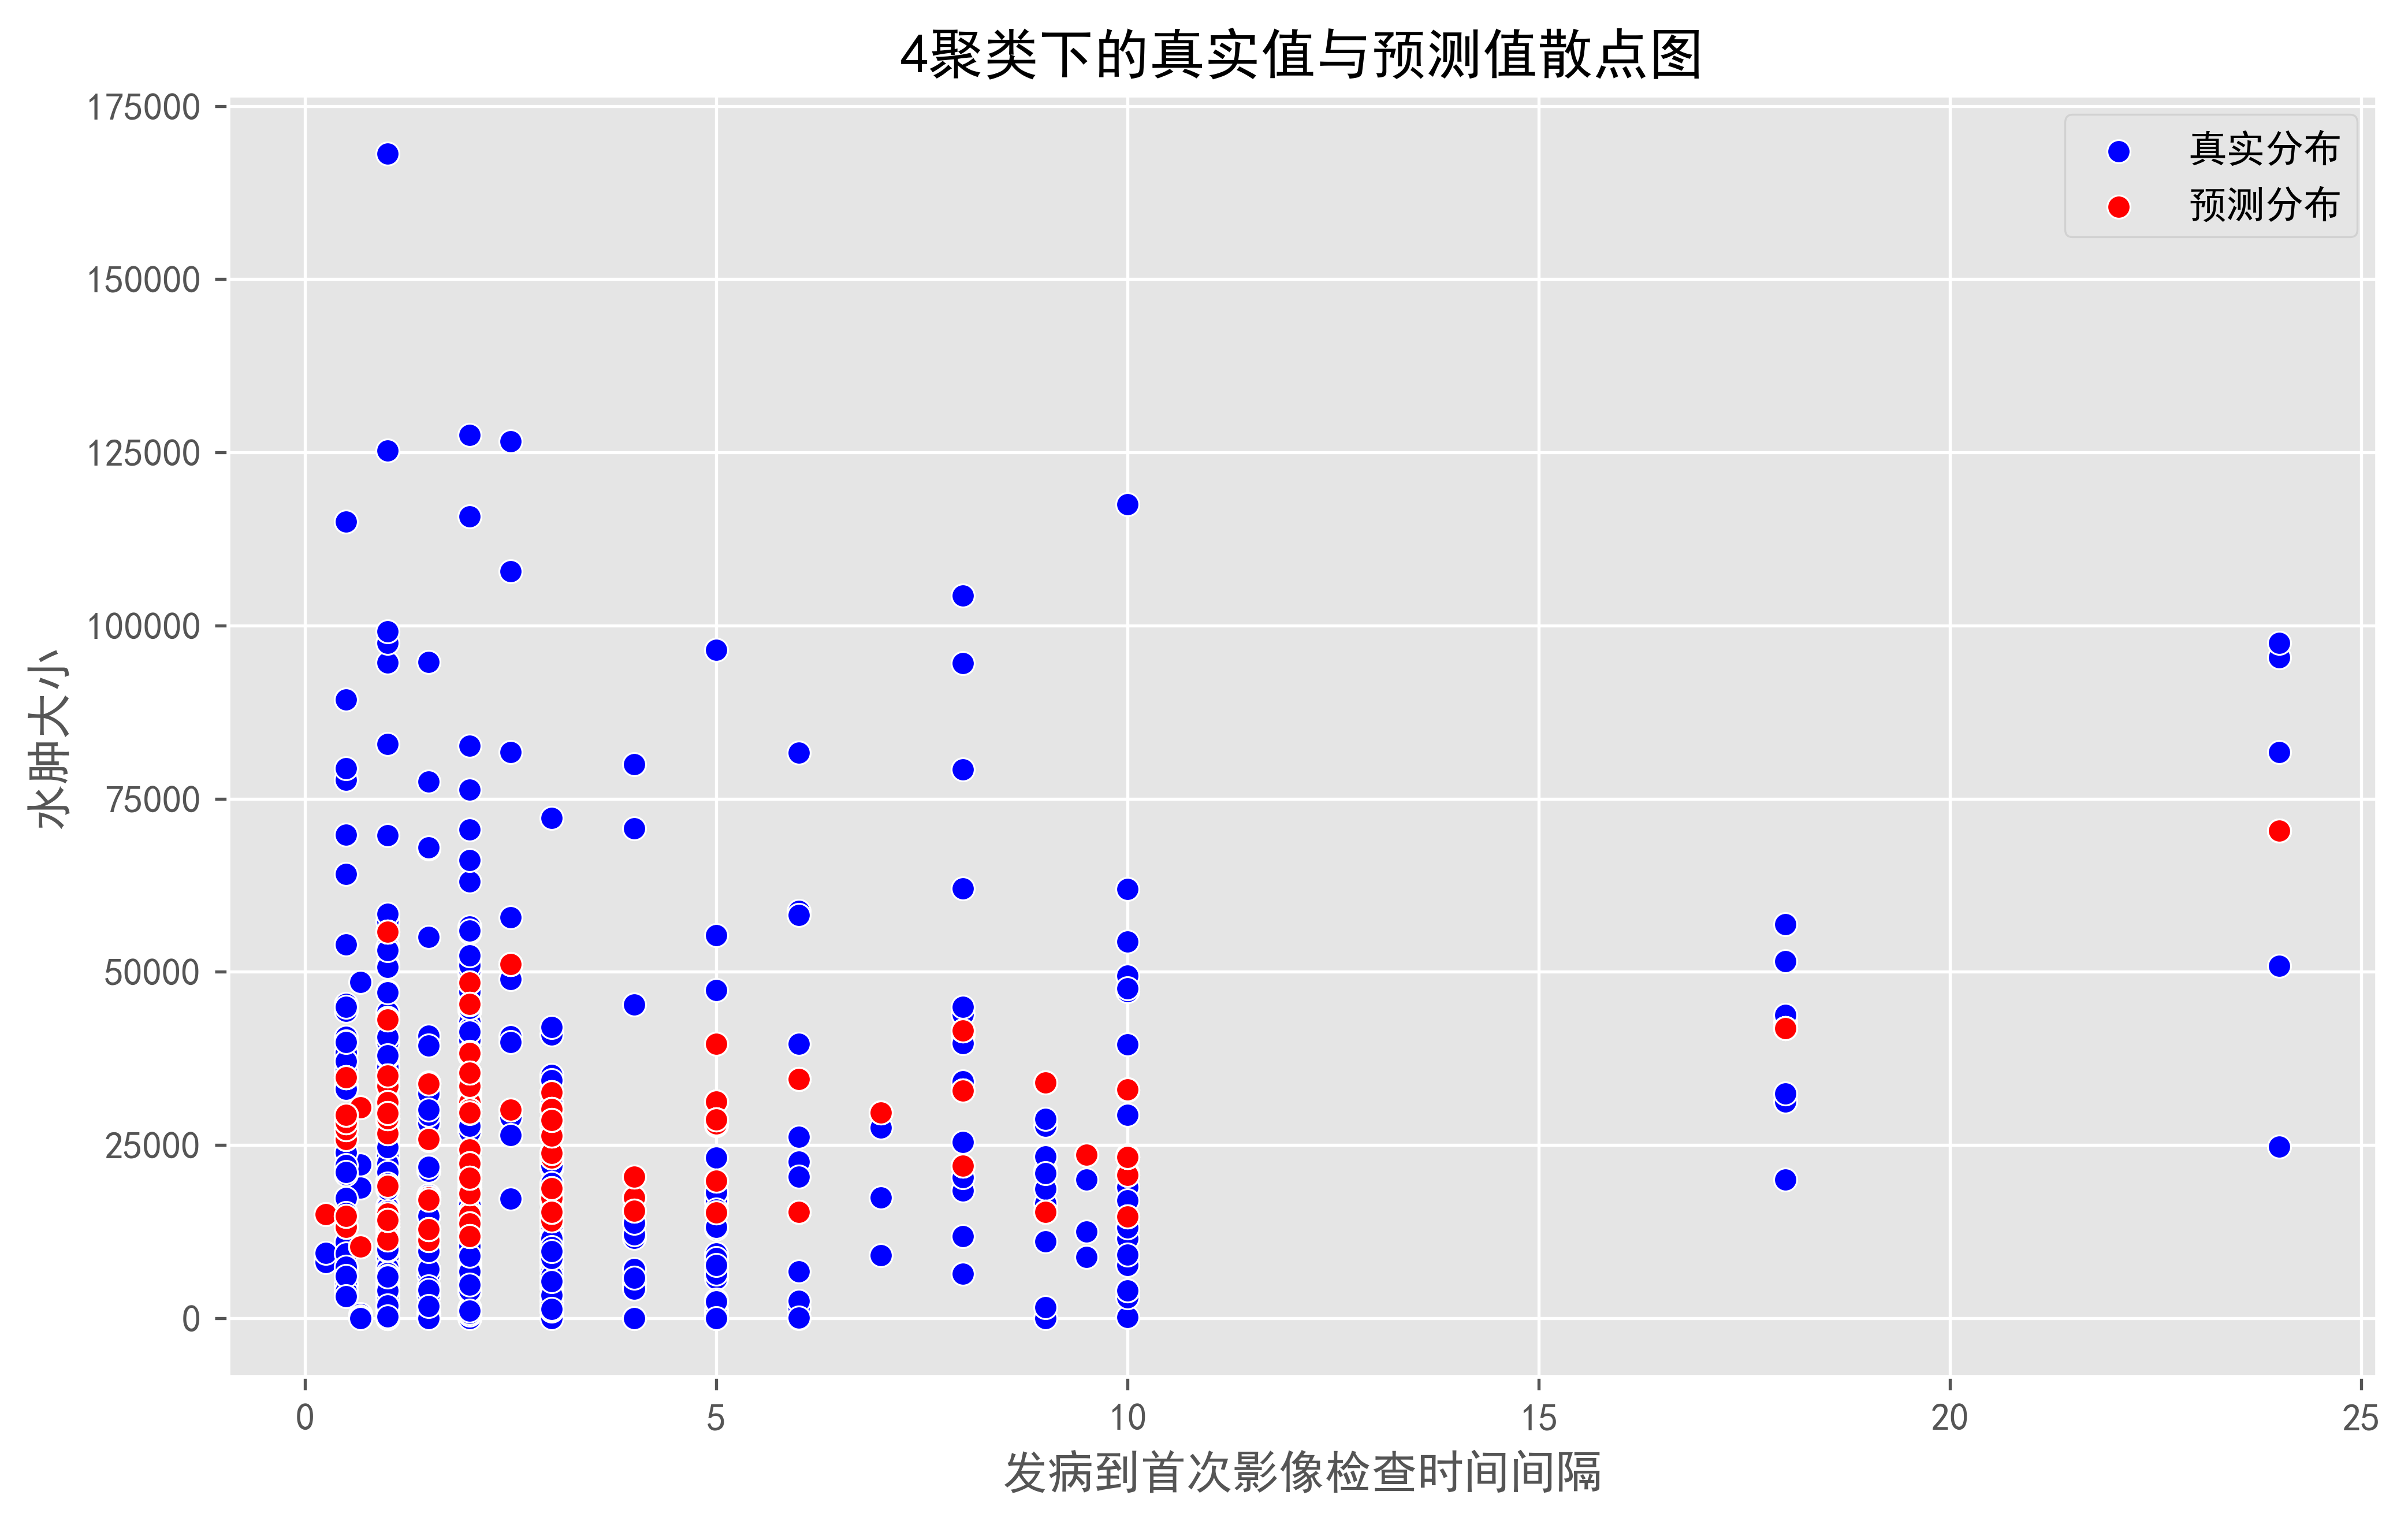
\includegraphics[width = 0.76\linewidth]{figures/q2_b_cluster_4_scatter.png}
    \caption{四聚类后的拟合散点图}
    \label{fig:聚类后的拟合散点图}
\end{figure}

分析数据易知,相较于聚类前模型对患者水肿体积大小的拟合曲线,聚类后曲线的拟合残差RMSE由25670.456降至了15740.167,即模型效果提升了36.6\%。

\subsection{第三问模型的建立与求解}
从数学模型的角度来看,分析不同治疗方法对水肿体积进展模式的影响,属于分析不同因素对输出的影响。因此,我们可以建立不同因素与输出的关系的数学模型来分析它们的影响。
\subsubsection{因果推断法}
在医学研究中,我们经常需要确定某种治疗方法是否真的能够有效地减少水肿体积的进展\cite{苗旺2018因果推断的统计方法}。为了解决这个问题,我们可以使用因果推断的方法。因果推断是一种数学方法,用于确定某个事件是否导致了另一个事件。在我们的研究中,我们可以将治疗方法作为因,将水肿体积的进展作为果,然后使用因果推断的方法来确定不同治疗方法对于水肿体积进展的影响效果。

因果推断法的原理如下:\par
因果推断法原理基于一个原则,即一个变量的变化(假设为原因)会导致另一个变量的变化(假设为结果)。因果推断法的公式如下:
\begin{equation}
Y=\alpha+\beta X+\varepsilon
\end{equation}

其中, $Y$ 是因变量, $X$ 是自变量, $\alpha$ 是常数项, $\beta$ 表示自变量对因变量的影响程度, $\varepsilon$ 是误差项。 

\subsubsection{建模与求解}
在对患者水肿体积和不同治疗方法做因果推断之前,需要先对患者的基本信息、不同治疗措施应用与否等特征以及病情进展结果(如水肿变化率)做预处理。

{\bf 连续特征标准化:}为了减少患者信息中连续特征的数量级差异,使特征具有可比性,首先对患者的连续特征进行标准化处理。这里我们使用z-score标准化来消除连续特征间的量纲差异,z-score标准化的计算公式如下:
\begin{align}
z-score &= \frac{(x - \mu)}{\sigma} \\
\mu &= \frac{1}{n}\sum_{i=1}^{n}x_i \\
\sigma^2 &= \frac{1}{n-1}\sum_{i=1}^{n}(x_i - \bar{x})^2 
\end{align}

其中,$n$表示数据的样本大小,$x$表示原始数据;$\mu$表示表示数据的平均值,即样本均值;$\sigma$表示数据的标准差,即样本标准差。
{\bf 线性回归:}建立线性回归模型,以病情进展结果(水肿体积变化率)为因变量,治疗措施为自变量,控制其他特征(年龄、性别等)。使用这些特征来拟合治疗效应,并计算RMSE评估模型拟合优度。
{\bf 两独立样本t检验:}
两独立样本均数差异的t检验(two-sample t-test)是一种常用的假设检验方法,用于比较两个样本的均值是否具有显著差异。因此,可以根据平均值差异的大小和P值来判断治疗措施的效果。

t检验的基本原理是假设两个样本来自具有相同均值的正态分布,并检验样本均值是否存在显著差异。如果样本均值存在显著差异,则可以拒绝原假设,即认为两个样本之间存在显著差异。 t检验的公式如下:

在两独立样本t检验中,我们需要比较两个样本的均值是否相等。假设样本2的观测值为$y$,样本2的均值$μ_2$,样本2的标准差$sigama_2$,则两样本t检验的原理和公式如下:
\begin{align}
t &= \frac{\bar{x} - \bar{y}}{s} \\
s^2 &= \frac{(\bar{x} - \bar{y})^2}{n_1-1} + \frac{(\bar{x} - \bar{y})^2}{n_2-1} \\
df &= n_1 + n_2 - 2 \\
p &= P(t > |t|) \
\end{align}

其中,$\bar{x}$ 和 $\bar{y}$ 分别是样本1和样本2的均值,$s$是两个样本的标准差之和,$d f$是自由度,$p$是双尾检验的概率值。

{\bf 结果展示:}在通过两独立样本t检验计算出两组样本间的差异值之后,计算两组样本间的平均值差异,并根据平均值差异的大小和P值来判断治疗措施的效果。检验结果如表\ref{tab:t检验}所示。
\begin{table}[ht]
\centering
\caption{两独立样本t检验结果}
\label{tab:t检验}
\fontsize{11}{9}\selectfont
\renewcommand\tabcolsep{6pt}
{

\begin{tabular}{cccc}
\toprule[1.2pt]
治疗方法    & t值           & p值          & RMSE         \\ \hline
脑室引流    & -3.996477521 & 9.83845E-05 & 10.85092637  \\
止血治疗    & 2.215551266  & 0.028152135 & -3.283633053 \\
降颅压治疗   & -0.631849939 & 0.5283981   & 0.974667795  \\
降压治疗    & -1.127355326 & 0.261301413 & 2.393760777  \\
镇静、镇痛治疗 & -1.539470021 & 0.125689914 & 2.200534668  \\
止吐护胃    & 0.076988611  & 0.93873001  & -0.243611368 \\
营养神经    & -0.32141552  & 0.748320317 & 1.016726442  \\ \bottomrule[1.2pt]
\end{tabular}}
\end{table}

在我们的研究中,我们发现脑室引流组和对照组之间存在显著差异,p值非常小(0.00025),T统计量为负值(-3.7664),平均数差为正值(11.9008)。这些数据表明,脑室引流组的意识障碍程度显著低于对照组。因此,脑室引流治疗可以有效降低意识障碍程度。

相比之下,止血治疗可能会导致轻微的增加意识障碍程度,p值较小(0.00527),T统计量为正值(2.83855),平均数差为负值(-5.46171)。虽然这种差异可能看起来很小,但我们需要考虑到p值较小可能是由于样本大小不足导致的。因此,我们需要进一步研究以确定止血治疗的实际效果。

其他治疗方法(如降颅压、降压、镇静镇痛等)没有显示出明显的疗效,p值较大,一般大于0.05。这表明这些治疗方法在治疗组和对照组之间没有显著的效应。

\subsection{第四问模型的建立与求解}
研究血肿体积、水肿体积及治疗方法三者之间的关系有助于深入理解脑损伤的病理生理过程和治疗效果,通过了解血肿体积与水肿体积之间的关系、血肿体积与治疗方法之间的关系以及水肿体积与治疗方法之间的关系,可以为临床实践提供有价值的指导,帮助医生为患者制定个体化的治疗方案。

为了进一步分析研究血肿体积、水肿体积及治疗方法三者之间的关系,我们分别选择使用时间序列相关分析法、两独立样本t检验法对三者间的关系一一分析。

\subsubsection{时间序列相关性分析}
时间序列相关性分析是研究时间序列数据中各数据点与时间之间的依赖关系,即数据点随时间变化的规律\cite{丁明2005基于时间序列分析的风电场风速预测模型}。在时间序列相关性分析中,常用的公式是自相关函数(Autocorrelation Function,ACF)和偏自相关函数(Partial Autocorrelation Function,PACF)\cite{liu2012comparison}。

自相关函数描述了时间序列中前一时间点与当前时间点之间的相关性,其公式为:
\begin{equation}
ACF(k) = E[(Y_t - Y_m)(Y_{t+k} - Y_m)]
\end{equation}

其中,$Y_t$表示时间序列中第t个观测值,$Y_m$表示时间序列中第m个观测值,E表示期望值。k表示自相关函数的阶数,即需要计算的时间点之间的距离。ACF(0)表示时间序列自身与当前时间点之间的相关性,ACF(1)表示时间序列自身与下一个时间点之间的相关性,以此类推。

偏自相关函数描述了时间序列中除了前一时间点与当前时间点之间的相关性外,还存在滞后一阶的偏差影响。其公式为:
\begin{equation}
PACF(k) = E[(Y_t - Y_m)(Y_{t+k} - Y_{m-k})] - E[(Y_t - Y_m)(Y_{t+k-1} - Y_{m-1})]
\end{equation}

其中,$m-k$表示偏自相关函数的阶数,即需要计算的时间点之间的距离。PACF(0)表示时间序列自身与当前时间点之间的相关性,PACF(1)表示时间序列自身与下一个时间点之间的相关性,以此类推。

通过自相关函数和偏自相关函数可以分析时间序列的长期依赖关系和周期性变化规律,为时间序列数据的分析和预测提供依据。

\subsubsection{血肿、水肿相关性分析}
在对患者血肿体积和水肿体积的关系进行分析时,我们沿用第二小问中对全体患者聚类的亚组结果。并分别对四个亚组的血肿体积、水肿体积关系做时间序列相关性分析。将
四个亚组的患者信息分别带入时间序列相关性分析模型,得到各组患者血肿体积和水肿体积的相关系数如表\ref{tab:血肿水肿相关性}所示。
\begin{table}[ht]
\centering
\caption{各亚组血肿体积和水肿体积的相关系数表}
\label{tab:血肿水肿相关性}
\fontsize{11}{9}\selectfont
\renewcommand\tabcolsep{6pt}
{
\begin{tabular}{cc}
\toprule[1.2pt]
亚组类别 & HM\_volume和ED\_volume的相关系数 \\ \hline
0    & 0.256879203                \\
1    & 0.121319768                \\
2    & 0.126008688                \\
3    & 0.225407361                \\ \bottomrule[1.2pt]
\end{tabular}}
\end{table}

通过对四类患者的血肿体积和水肿体积进行相关性分析,得出每类患者的相关系数。这些系数用于衡量两个变量之间的线性关系强度和方向。

对于第0类患者,HM\_volume和ED\_volume的相关系数为0.2568792029800091,属于中等强度正相关,表明血肿体积增加通常会导致水肿体积增加。

对于第1类患者,相关系数为0.12131976804052762,表明血肿体积和水肿体积之间存在弱的负相关关系。这可能是因为该类患者的血肿体积较小,对水肿体积的影响较小。

对于第2类和第3类患者,相关系数分别为0.126008687633567和0.22540736135529715,均属于较弱相关,表明血肿体积和水肿体积之间存在中等强度的正相关关系。

\subsubsection{水肿、治疗方法的因果推断分析}
在第三小问种,我们研究了不同治疗方法对水肿体积进展模式的影响。在这一环节中,我们将进一步的研究不同治疗方法,对不同亚组患者水肿体积进展模式的影响。同时在研究方法上,我们沿用第三小问建立的因果推断模型做细致研究。

将四个亚组患者预处理过后的信息分别带入因果推断模型,得到各组别患者治疗方法和水肿体积的检验结果如表\ref{tab:各亚组治疗方法水肿}所示。
\begin{table}[ht]
\centering
\caption{各亚组不同治疗方法对水肿体积进展模式的影响}
\label{tab:各亚组治疗方法水肿}
\fontsize{11}{9}\selectfont
\renewcommand\tabcolsep{6pt}
{
\begin{tabular}{ccccc}
\toprule[1.2pt]
治疗方法         & 亚族类别         & t值           & p值           & 平均数差         \\ \midrule
脑室引流:        & 0            & 0.264948318  & 0.79554551   & -0.220757479 \\
镇静、镇痛治疗:     & 0            & -1.476222738 & 0.165637734  & 1.330724984  \\
\textbf{...} & \textbf{...} & \textbf{...} & \textbf{...} & \textbf{...} \\
降压治疗         & 1            & -0.827261589 & 0.412454283  & 2.664417911  \\
\textbf{...} & \textbf{...} & \textbf{...} & \textbf{...} & \textbf{...} \\
镇静、镇痛治疗:     & 2            & NAN          & NAN          & 0.179997761  \\
\textbf{...} & \textbf{...} & \textbf{...} & \textbf{...} & \textbf{...} \\
营养神经:        & 3            & -0.023796308 & 0.981150241  & 0.160024917  \\ \bottomrule[1.2pt]
\end{tabular}}
\end{table}

经过两独立样本t检验的研究,对于患者采用的不同治疗方法与水肿体积大小之间的关系得到了以下结论:



\begin{enumerate}
    \item 对于编号为0、1、2的亚组而言,所采用的治疗方法均没有显示出明显的疗效,p值较大,大于0.05。这表明这些治疗方法在治疗组和对照组之间没有显著的效应;
    \item 对于编号为3的亚组而言,止血治疗可能会导致轻微的增加意识障碍程度,p值较小(0.0146),T统计量为正值(2.56),平均数差为负值(-11.735),即止血治疗可以对患者水肿体积的减小有着不可忽视的抑制效果。
\end{enumerate}

综上所述,不同治疗方法对患者的水肿体积大小有显著影响。对于采用止血治疗的患者,水肿体积大小存在统计学差异;而对于采用降颅压治疗的患者,水肿体积大小没有显著差异。因此,在治疗过程中需要根据患者的具体情况选择合适的治疗方法,以降低水肿对患者的影响。


\subsubsection{血肿、治疗方法的因果推断分析}
在这一环节,我们需要研究患者血肿体积和不同治疗方法之间的关系,和研究患者水肿体积和不同治疗方法之间关系的目标类似。两者均是以研究多组别自变量和单组别因变量之间关系为任务,因此在对患者血肿体积和不同治疗方法之间的关系进行研究时,我们依然沿用前文中所建立的因果推断模型。同时,在对患者信息进行分析时,沿用第二小问中对患者的亚分组结果,对不同亚组患者血肿体积和不同治疗方法之间的关系做细致化的研究。

将四个亚组患者预处理过后的信息分别带入因果推断模型,得到各组别患者治疗方法和血肿体积的检验结果如表\ref{tab:各亚组不同治疗方法血肿}所示。
\begin{table}[ht]
\centering
\caption{各亚组不同治疗方法对血肿体积进展模式的影响}
\label{tab:各亚组不同治疗方法血肿}
\fontsize{11}{9}\selectfont
\renewcommand\tabcolsep{6pt}
{
\begin{tabular}{ccccc}
\toprule[1.2pt]
治疗方法       & 亚族类别       & t值         & p值         & 平均数差       \\ \midrule
脑室引流:      & 0          & -0.20787   & 0.838817   & 0.050949   \\
\textbf{…} & \textbf{…} & \textbf{…} & \textbf{…} & \textbf{…} \\
止血治疗       & 1          & 1.125985   & 0.266141   & -0.35201   \\
降颅压治疗      & 1          & 1.450096   & 0.153966   & -0.40649   \\
\textbf{…} & \textbf{…} & \textbf{…} & \textbf{…} & \textbf{…} \\
镇静、镇痛治疗:   & 2          & NAN        & NAN        & 0.294945   \\
\textbf{…} & \textbf{…} & \textbf{…} & \textbf{…} & \textbf{…} \\
止吐护胃       & 3          & -0.16928   & 0.866548   & 0.11999    \\
营养神经       & 3          & -0.79125   & 0.434126   & 0.460704   \\ \bottomrule[1.2pt]
\end{tabular}}
\end{table}

经过两独立样本t检验的研究,对于患者采用的不同治疗方法与血肿体积大小之间的关系得到了以下结论:



\begin{enumerate}
    \item 对于编号为0的亚组而言,镇静、镇痛治疗可能会导致轻微的降低意识障碍程度,p值相对较小(0.0813668971466179)。由于患者采用的治疗方法较少,数据样本集不足以支持检验结果的产生,因此,需要更多的数据来进一步研究其它治疗方法对该亚组患者血肿体积大小的影响;
    \item 对于编号为1的亚组而言,所采用的治疗方法均没有显示出明显的疗效,p值较大,大于0.05。这表明这些治疗方法在治疗组和对照组之间没有显著的效应;
    \item 对于编号为2、3的亚组而言,所采用的治疗方法均没有显示出明显的疗效,p值较大,大于0.05。这表明这些治疗方法在治疗组和对照组之间同样没有显著的效应。

\end{enumerate}

综上所述,不同治疗方法对患者的血肿体积大小有一定影响。对于采用止血治疗的患者,血肿体积大小存在统计学差异。因此,在治疗过程中需要根据患者的具体情况选择合适的治疗方法,以降低血肿对患者的影响。

\section{问题三建模与求解}
\subsection{问题分析}
出血性脑卒中患者的预后预测及关键因素探索有助于提高患者的生存率和生活质量,为临床相关决策提供依据。通过探索患者的个人史、疾病史、治疗方法及影像特征等关键因素,可以为患者提供更精准、个性化的治疗方案和护理措施。

在本问中,我们一共要完成三项任务:
\begin{enumerate}
    \item 对前一百名患者的信息进行匹配,然后根据患者的个人史、疾病史、发病相关信息和首次影像结果,构建预测模型,预测患者90天mRS评分;
    \item 根据前100个患者的所有已知临床、治疗信息和影像(首次和随访)结果,预测所有含随访影像检查的患者90天mRS评分;
    \item 建立合适的数学模型,分析出血性脑卒中患者的预后(90天mRS)和个人史、疾病史、治疗方法及影像特征等关联关系,并依此为临床相关决策提供建议。

\end{enumerate}
    
\subsection{第一问模型的建立与求解}
在本项任务中,我们需要通过患者的个人史、疾病史、发病相关(“表1”字段E至W)及首次影像结果(表2,表3中相关字段)构建预测模型,预测患者(sub001至sub160)90天mRS评分。
我们采用深度森林对患者90天mRS评分进行预测。首先我们先对数据进行了处理,对分类特征进行one-hot编码,连续特征归一化到[0,1]范围。
\subsubsection{深度森林}
深度森林是一种集成学习方法,它组合了多个决策树来进行预测\cite{zhou2019deep}。在这里,我们将使用深度森林模型进行预测。每个决策树将根据患者的个人史、疾病史、发病相关特征以及首次影像结果来进行预测。
首先,深度森林模型的整体预测可以表示为:
\begin{equation}
Y_i = F(X_i)
\end{equation}
其中,$Y_i$是对第i个患者的90天mRS评分的预测值。$X_i$是包含第i个患者的特征集,包括个人史、疾病史、发病相关特征以及首次影像结果。$F$是深度森林模型,它是多个决策树的集成。
深度森林模型中的每个决策树的预测可以表示为:
\begin{equation}
F_k(X_i) = \sum_{j=1}^{J_k}c_{kj}·I(X_i\epsilon R_{kj})
\end{equation}
其中$F_k(X_i)$是第k棵树的测值。$J_k$是第k棵树的叶节点数量。$c_{kj}$是第k棵树的第j个叶节点的值。$I(X_i\epsilon R_{kj})$是一个指示函数,如果第i个患者的特征集$X_i$位于第k棵树的第j个叶节点$R_{kj}$内,则值为1,否则为0。
最终的预测值是所有决策树的预测值的平均值:
\begin{equation}
Y_i = \frac{1}{K}\sum_{k=1}^{K}F_k(X_i)
\end{equation}
其中, K是深度森林中决策树的数量。

\subsubsection{模型的求解}
如上文所述数据预处理方案,本文采用深度森林方式对首次影响检查数据和90天mRS评分进行建模,同样,我们首先将所有特征作为自变量,将90天mRS作为因变量进行拟合,通过该模型求解得到变量的重要程度,并选取了前十个重要的变量进行模型的二次拟合,我们的实验结果如表\ref{tab:q31}所示。其中训练集和测试集为前100个病人ID按照8:2的比例进行随机采样(我们的具体结果详见补充材料中的表4)。

% Please add the following required packages to your document preamble:
% \usepackage{multirow}
\begin{table}[ht]
\centering
\caption{问题三第一小问求解结果}
\label{tab:q31}
\fontsize{11}{9}\selectfont
    \renewcommand\tabcolsep{6pt}
    {
\begin{tabular}{lcccc}
\toprule[1.2pt]
\multicolumn{1}{c}{\multirow{2}{*}{}} & \multicolumn{2}{c}{一次拟合} & \multicolumn{2}{c}{二次拟合} \\
\multicolumn{1}{c}{}                  & 训练精度        & 测试精度       & 训练精度        & 测试精度       \\ \hline

DeepForest (Ours)                      & 0.85        & 0.45       & 0.87        & 0.55       \\
LightGBMXT                            & 0.67        & 0.35       & 0.70         & 0.40        \\ \bottomrule[1.2pt]
\end{tabular}}
\end{table}

从表中可以看出,我们采用的方案取得了最优的性能,同时我们发现,进行特征筛选后进行训练,模型的训练精度差异不大,但是在测试集上的精度有了较大的提升,这说明过多的特征容易造成模型的过拟合,导致在测试集上的精度下降较多。因此进行二次的特征筛选是很有必要的。
\subsection{第二问模型的建立与求解}
在本问中我们将根据前100个患者(sub001至sub100)所有临床、治疗(表1字段E到W)、表2以及表3的影像(首次+随访)结果,去预测所有含随访影像检查的患者(sub001至sub100,sub131至sub160)90天mRS评分。本问多引入了随访影像结果这一因素,其与首次影像结果存在时间层面的关联,因此再数据处理阶段我们添加了时间间断字段来引入了时间相关联的因素。我们通过建模LSTM网络对所有含随访影像检查的患者90天mRS进行预测。
\subsubsection{LSTM模型}
LSTM网络是一种常用于处理序列数据的循环神经网络(RNN)变种。LSTM网络的关键在于它的记忆单元和门控机制,使其能够更好的捕捉和处理长期依赖性,适用于建立各种序列建模任务。
LSTM的主要组成结构为输入门$i_t$、遗忘门$f_t$和输出门$o_t$。LSTM的核心是细胞状态,它可以被看作是网络的"记忆"。细胞状态可以在长期时间内保持信息,允许网络存储和访问过去的信息。
\begin{enumerate}
    \item LSTM单元的输入门(input gate)
    输入门决定要更新细胞状态的程度。它的计算通常由以下公式表示:$i_t = \sigma(W_i \cdot [h_{t-1}, x_t] + b_i)$。
    \item LSTM单元的遗忘门:
    遗忘门决定要从细胞状态中忘记多少信息。它的计算通常由以下公式表示:$f_t = \sigma(W_f \cdot [h_{t-1}, x_t] + b_f)$。
    \item 更新细胞状态:
    细胞状态的更新通过以下公式完成:$C_t = C_t + C_t$。 
    \item LSTM单元的输出门:
    输出门决定要输出多少细胞状态的信息。它的计算通常由以下公式表示:$o_t = \sigma(W_o \cdot [h_{t-1}, x_t] + b_o)$。
    \item 隐藏状态的更新:
    最后,使用输出门和更新后的细胞状态来计算当前时间步的隐藏状态:$h_t = o_t \cdot \tanh(C_t)$。
\end{enumerate}
\subsubsection{模型的求解}
由于本问使用了额外多次的随访结果,随访之间存在着时间关联性,因此,本问采用更加适合时序建模的LSTM模型对本问进行建模,和上一小问同样的,我们采用了二次拟合的方式进行建模,首先对所有特征进行拟合,在筛选出影响程度较大的十个变量,通过这十个变量进行二次拟合,我们的模型结果如表\ref{tab:q32}所示。

% Please add the following required packages to your document preamble:
% \usepackage{multirow}
\begin{table}[ht]
\centering
\caption{问题三第二小问求解结果}
\label{tab:q32}
\fontsize{11}{9}\selectfont
    \renewcommand\tabcolsep{6pt}
    {
\begin{tabular}{lcccc}
\toprule[1.2pt]
\multirow{2}{*}{} & \multicolumn{2}{c}{一次拟合} & \multicolumn{2}{c}{二次拟合} \\
                  & 训练精度        & 测试精度       & 训练精度        & 测试精度       \\ \hline
LSTM (Ours)              & 0.968       & 0.840      & 0.995       & 0.975      \\
LightGBMXT        & 0.923       & 0.815      & 0.985       & 0.951      \\ \bottomrule[1.2pt]
\end{tabular}}
\end{table}

我们发现,在采用多次随访结果进行拟合后,测试精度和训练精度都达到了一个很高的水平,这表明对于水肿和血肿的建模来说,长时序的特征更加有利于对疾病程度的判断,相较于仅仅凭借首次影像的诊断,多次诊断结果精度提升了将近一倍。因此,病患有必要进行定期的检查一遍医生做出正确的决断。

\subsection{第三问模型的建立与求解}
在这任务中我们需要通过分析出血性患者的预后与其个人史、疾病史、治疗方法以及影像特征之间的关系来去更好的提供临床方面决策的建议,以此来帮助医疗的专业人员能更加了解影响预后的种种因素,并在为患者提供针对性的治疗方案。我们将通过两种方案来分析mRS影响因素。
\subsubsection{相关性分析}
我们通过计算病患个人信息、临床指标和CT影像信息与病患预后的Pearson相关系数来进行分析。对于每个特征$x_i$,计算其与目标变量$y$(即90天mRS评分)的Pearson相关系数:
\begin{equation}
r_{x_iy} = \frac{\sum_{j=1}^{N}(x_{ij}-\bar{x_i})(y_j-\bar{y})}{\sqrt{\sum_{j=1}^{N}(x_{ij}-\bar{x_i})^2}\sqrt{\sum_{j=1}^{N}(y_j-\bar{y})^2}}
\end{equation}
其中,$\bar{x_i}$,$\bar{y}$分别为$x_i$,$y$的平均值。$N$为样本数量。

我们选取了前10个相关性系数高的特征对其进行分析。从表\ref{tab:影响病患预后的前10个特征}可以看出病患的血肿指标很大程度影响着90天mRS。血肿的表面面积、体积、最大二维直径、轴长等,这些与病灶大小、扩展范围相关,与预后评分正相关。糖尿病史和冠心病史与预后也存在正相关,可能是由于基础疾病会对神经系统造成影响。
综合来看,病灶图像特征是影响预后最关键的因素之一,但不能忽视基础疾病和健康状况的综合影响。

\begin{table}[ht]
    \centering
    \caption{影响病患预后的特征(TOP10)}
    \label{tab:影响病患预后的前10个特征}
    \fontsize{11}{9}\selectfont
    \renewcommand\tabcolsep{6pt}
    {
    \begin{tabular}{cc}
    \toprule[1.2pt]
    Feature      &    Correlation         \\
    \midrule
    original\_shape\_SurfaceArea\_Hemo &  
     0.39930563864819446 \\
    HM\_volume  &  0.3855776316216518  \\
    original\_shape\_Maximum2DDiameterColumn\_Hemo &   0.38484300696888557 \\
    original\_shape\_LeastAxisLength\_Hemo         &   0.3726962035382604  \\
    original\_shape\_VoxelVolume\_Hemo             &   0.3561706236369382  \\
    original\_shape\_MeshVolume\_Hemo              &   0.3561098037359607  \\
    original\_shape\_MajorAxisLength\_Hemo         &   0.34009470239168677 \\
    糖尿病史       &   0.3133283408213977  \\
    冠心病史       &   0.3131265691541535  \\
    NCCT\_original\_firstorder\_Range\_ED        &   0.30870457107435795 \\
    \bottomrule[1.2pt]
    \end{tabular}
    }
\end{table}


\subsubsection{特征重要性}
我们使用LightGBM等机器学习模型可以输出特征重要度\cite{徐少成2018基于随机森林的加权特征选择算法},这些特征重要度指标通常用于衡量特征对目标变量(在这种情况下是90天mRS评分)的贡献程度。一般来说,特征重要度分数越高,表明该特征对预测目标变量的贡献越大。以下是一种数学建模的方式来描述特征重要性的计算过程:
我们通过训练好的模型计算特征重要度分数。对于一个特征 $X_i$,它的特征重要度分数$FI$可以表示为:
\begin{equation}
FI(X_i)=\frac{\sum_{j}Gain(X_i,j)\cdot I(X_i, j)} {\sum_{j}Gain(X_i,j)}
\end{equation}

其中,$\text{FI}(X_i)$ 表示特征 $X_i$ 的特征重要度分数。
$\text{Gain}(X_i, j)$ 表示特征 $X_i$ 在模型的节点 $j$ 分裂时带来的增益,通常可以通过基尼不纯度或均方误差的减小来衡量。
$I(X_i, j)$ 是一个指示函数,如果特征 $X_i$ 在节点 $j$ 分裂中使用了,则为1,否则为0。
$N$ 是总的节点数。
最后,我们根据特征重要度分数对所有特征进行排序,选择前几名的特征,这些特征被认为对于预测90天mRS评分的贡献最高。
我们也根据特征重要度分数对影响患者预后因素进行了进一步分析。
%表\ref{tab:第一问模型特征重要性(Top10)}给出了第一个模型训练好后所得到的重要性前十的特征,通过我们的分析我们得出以下点结论:
%\begin{enumerate}
%    \item 最重要的特征是图像灰度的熵(NCCT\_original\_firstorder\_Entropy\_x),反映病灶组织异质性。
%    \item 血肿在左后动脉区的比例(HM\_PCA\_L\_Ratio)排第二,提示该部位血肿与预后相关。
%    \item 低血压和左前动脉水肿比例(ED\_ACA\_L\_Ratio)也较重要,血流动力学和水肿程度影响大。
%    \item 年龄因素也很大程度得印象病患的预后,年纪越大的病患身体的机能会比较差,这会导致恢复缓慢,治疗效果也会大打折扣。
%    \item 影像形态特征如表面面积、体积、轴长等对病灶大小也有一定影响。影像形态一定程度上代表着疾病发展的现状,是最直观判断病情发展好坏的指标。
%\end{enumerate}
%总体来看,本组患者预后主要与病灶部位、年龄、血流动力学相关。

表\ref{tab:第二问模型特征重要性(Top10)}给出了模型训练好后所得到的重要性前十得特征,我们可以得出以下几点:
\begin{enumerate}
    \item 最重要的特征是糖尿病史,提示糖尿病作为基础疾病会对预后产生重要影响。糖尿病会降低病患的免疫力,疾病所造成的损害不能及时的进行自我修复,导致病情恢复缓慢甚至变得更为严重。
    \item 右前动脉血肿分布比例(HM\_ACA\_R\_Ratio)也较重要,血肿所在位置与严重程度相关。
    \item 发病到影像时间间隔排第三,发病越慢救治及时程度较好。
    \item 年龄、低血压、吸烟史等个人信息特征位列前列。
\end{enumerate}


%\begin{table}[ht]
%    \centering
%    \caption{第一问模型特征重要性(Top10)}
%    \label{tab:第一问模型特征重要性(Top10)}
%    \fontsize{11}{9}\selectfont
%    \renewcommand\tabcolsep{6pt}
%    {
%   \begin{tabular}{ccccccc}
%    \toprule[1.2pt]
%   feature                                           & importance & stddev & p\_value & n & p99\_high & p99\_low \\
%   \midrule
%ED\_ACA\_L\_Ratio                                 & 0.08       & 0.02   & 0.00     & 5 & 0.12      & 0.04     \\
%低压                                                & 0.08       & 0.01   & 0.00     & 5 & 0.09      & 0.06     \\
%HM\_PCA\_L\_Ratio                                 & 0.07       & 0.02   & 0.00     & 5 & 0.11      & 0.03     \\
%ED\_PCA\_L\_Ratio                                 & 0.04       & 0.02   & 0.00     & 5 & 0.08      & 0.00     \\
%年龄                                                & 0.04       & 0.01   & 0.00     & 5 & 0.07      & 0.02     \\
%HM\_ACA\_R\_Ratio                                 & 0.04       & 0.01   & 0.00     & 5 & 0.06      & 0.02     \\
%HM\_ACA\_L\_Ratio                                 & 0.04       & 0.01   & 0.00     & 5 & 0.06      & 0.02     \\
%NCCT\_original\_firstorder\_Uniformity\_y         & 0.03       & 0.01   & 0.00     & 5 & 0.06      & 0.01     \\
%NCCT\_original\_firstorder\_InterquartileRange\_x & 0.03       & 0.01   & 0.00     & 5 & 0.05      & 0.02     \\
%original\_shape\_Elongation\_x                    & 0.03       & 0.01   & 0.00     & 5 & 0.04      & 0.02     \\
%    \bottomrule[1.2pt]
%    \end{tabular}
%    }
%\end{table}


\begin{table}[ht]
    \centering
    \caption{模型特征重要性(Top10)}
    \label{tab:第二问模型特征重要性(Top10)}
    \fontsize{11}{9}\selectfont
    \renewcommand\tabcolsep{6pt}
    {
    \begin{tabular}{ccccccc}
    \toprule[1.2pt]
   feature                                           & importance & stddev & p\_value & n & p99\_high & p99\_low \\
   \midrule
糖尿病史\_1                        & 0.03       & 0.00   & 0.00     & 5 & 0.04      & 0.02     \\
HM\_ACA\_R\_Ratio              & 0.03       & 0.00   & 0.00     & 5 & 0.03      & 0.02     \\
发病到首次影像检查时间间隔                  & 0.02       & 0.01   & 0.00     & 5 & 0.04      & 0.01     \\
房颤史\_1                         & 0.02       & 0.00   & 0.00     & 5 & 0.03      & 0.01     \\
吸烟史\_1                         & 0.02       & 0.00   & 0.00     & 5 & 0.03      & 0.01     \\
低压                             & 0.02       & 0.00   & 0.00     & 5 & 0.02      & 0.01     \\
年龄                             & 0.01       & 0.00   & 0.00     & 5 & 0.02      & 0.01     \\
止吐护胃\_1                        & 0.01       & 0      & 0.50     & 5 & 0.01      & 0.01     \\
original\_shape\_Flatness\_y   & 0.01       & 0.01   & 0.00     & 5 & 0.03      & 0.00     \\
original\_shape\_Elongation\_y & 0.01       & 0.01   & 0.00     & 5 & 0.03      & 0.00      \\
    \bottomrule[1.2pt]
    \end{tabular}
    }
\end{table}

\subsubsection{临床决策的建议}
分析上述feature importance结果,影响血性脑卒中患者预后90天mRS评分的重要特征包括糖尿病史、右前动脉血肿分布比例、发病到影像时间间隔、年龄、低血压和吸烟史等个人信息特征。

为了保证患者的身体健康情况,临床决策应该综合考虑以下几点:

\begin{enumerate}
    \item 针对有糖尿病史的患者,应加强对其糖尿病的管理和控制,包括合理控制血糖水平、定期检查、接受规范治疗等,以提高免疫功能和促进病情恢复;
    \item 对于血肿分布在右前动脉的患者,需要密切监测其病情变化,及时采取适当的治疗措施,包括手术、药物治疗等,以减轻血肿对脑组织的损害;
    \item 在治疗过程中,需要密切监测患者的病情变化,提供及时的治疗干预,包括药物治疗、康复训练等,以促进患者的康复;
    \item 在治疗过程中,需要根据患者的年龄、血压情况和吸烟史等个人信息特征进行个体化的治疗决策。年龄较大、低血压患者需要密切监测血压和相关生命体征,并给予适当的支持治疗;吸烟者应引导他们戒烟,以减少吸烟对血管造成的损害。

\end{enumerate}

换言之,临床决策应综合考虑患者的个人疾病史、血肿分布位置、治疗及时程度、年龄、血压、吸烟史等因素,制定个体化的治疗方案,以促进患者的康复和预防二次脑卒中的发生。

\clearpage
\section{模型评价}
\subsection{灵敏度分析}
本文涉及的大部分模型都不依赖于精细的调参,采用默认参数就能取得比较好的性能。然而,所提出的模型仍有部分需要人为调节,例如,亚类人群划分的聚类数,以及模型特征数量的选取等。因此,在这一部分,我们对这些设置进行灵敏度分析。

\subsubsection{聚类数目的灵敏度分析}
在第二问中,涉及到聚类数目的选择,本文的实验证明了在对患病人群进行聚类后,预测模型的指标会得到一定的提升,然而,聚类数量的选择对最终性能的增益仍然有一定的探索空间\cite{hamerly2003learning},因此,在这一部分我们划分了3-8个聚类数目,并对最终的预测结果进行评价。评价指标分成预测的性能和聚类的性能,其中预测的性能使用RMSE指标进行衡量,聚类的性能采用轮廓系数进行衡量,轮廓分数是一种聚类效果评估指标,用于衡量聚类的紧密度和分离度。它的计算方法如下:
\begin{itemize}
    \item 对于每个样本i,计算其与同一簇内所有其他样本的平均距离,记为a(i)。
    \item 对于样本i,计算其与最近不同簇内所有样本的平均距离,记为b(i)。
    \item 轮廓系数s(i)定义为:s(i) = (b(i) - a(i)) / max{a(i), b(i)}
\end{itemize}
最终的轮廓分数是所有样本的轮廓系数的平均值。轮廓分数的取值范围在-1到1之间:如果s(i)接近1,表示样本i聚类得很好,距离其同一簇内的其他样本较近,与不同簇的样本距离较远。我们的计算结果如表\ref{tab:cluster}和图\ref{fig:cluster}所示,
\begin{table}[ht]
\centering
\caption{聚类数量灵敏度分析,\textbf{黑体}表示最佳结果,\underline{下划线}表示次优结果}
\label{tab:cluster}
\fontsize{11}{9}\selectfont
    \renewcommand\tabcolsep{6pt}
    {
\begin{tabular}{lccccccc}
\toprule[1.2pt]
\textbf{聚类数}  & 2             & 3        & 4                 & 5        & 6        & 7        & 8        \\ \midrule
\textbf{聚类得分} & \textbf{0.67} & 0.56     & \underline{0.62}              & 0.56     & 0.57     & 0.53     & 0.54     \\
\textbf{RMSE} & 16828.78      & 16544.75 & \textbf{15740.17} & 16460.35 & 16197.40 & 16547.04 & \underline{16101.55} \\ \bottomrule[1.2pt]
\end{tabular}}
\end{table}

\begin{figure}[ht]
    \centering
    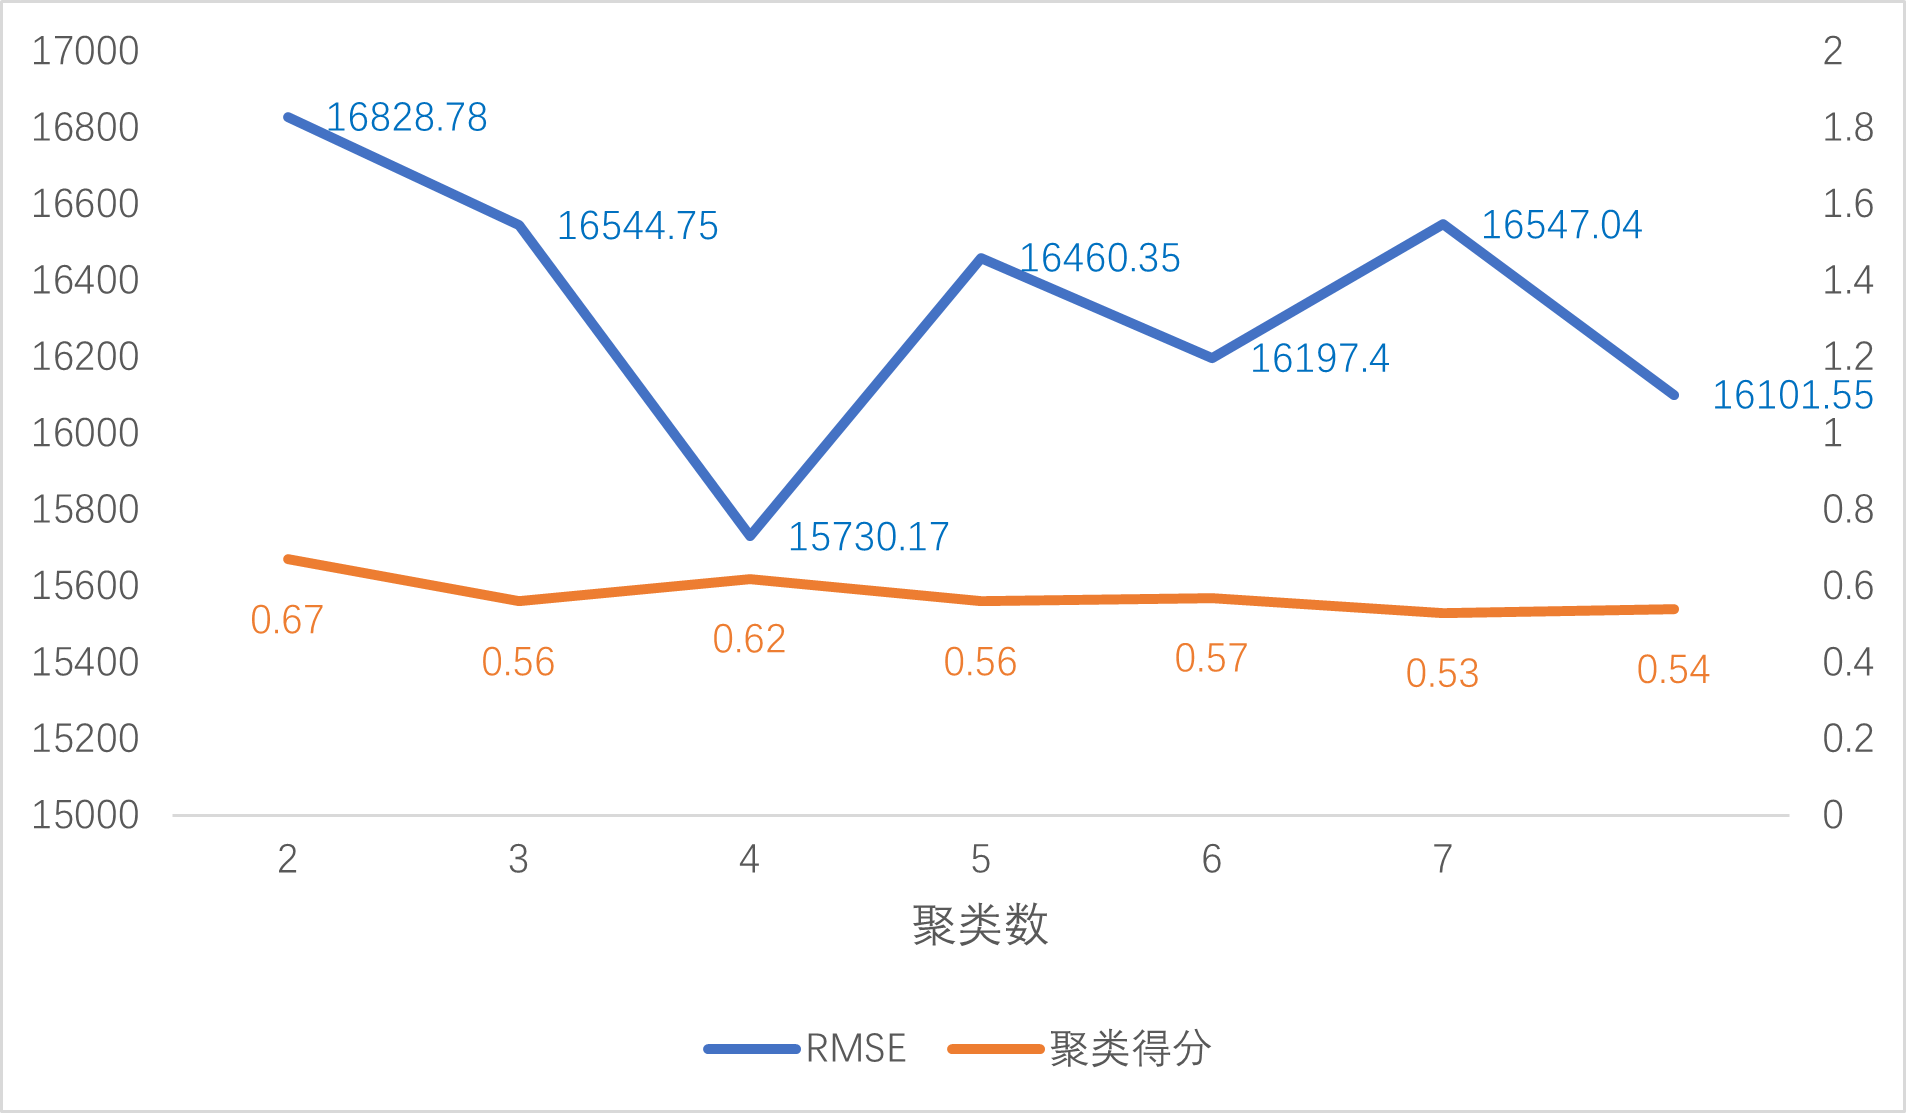
\includegraphics[width = 0.8\linewidth]{figures/7.11.png}
    \caption{聚类数量灵敏度分析}
    \label{fig:cluster}
\end{figure}
从表中的结果可以看出,我们的方案对于聚类数量的敏感度不高,调节聚类的数量无论是聚类的得分还是RMSE的预测指标变化都不太大,在预测水肿体积时表现了较强的鲁棒性。其中4聚类取得了次优的聚类得分和最优的预测得分,这说明聚类的好坏在一定程度上会影响到最后预测的RMSE值。

\subsubsection{模型特征数量的灵敏度分析}
在本文构建的模型中,对数据进行了降维,降维的方式通过计算特征重要性,然后选取前k个重要特种进行模型的进一步拟合,然后k作为一个超参数,需要进行人工调节,为此,和上一部分保持一致,我们仍采用第二问中的预测对k进行灵敏度分析,调节k的范围为5-19,和上一小节保持一致,我们采用聚类得分和预测得分衡量模型的综合性能,我们的灵敏度分析结果如表\ref{tab:feature}和图\ref{fig:feature}所示。

\begin{table}[ht]
\centering
\caption{特征数量灵敏度分析,\textbf{黑体}表示最佳结果,\underline{下划线}表示次优结果}
\label{tab:feature}
\fontsize{11}{9}\selectfont
    \renewcommand\tabcolsep{5pt}
    {
\begin{tabular}{lcccccccc}
\toprule[1.2pt]
\textbf{特征数量} & 5             & 7        & 9                 & 11       & 13       & 15       & 17       & 19       \\ \midrule
\textbf{聚类得分} & {0.62} & 0.62     & 0.62              & 0.62     & 0.62     & 0.62     & 0.62     & 0.62     \\
\textbf{RMSE} & 16235.80      & 16876.47 & \underline{15783.28} & 16641.38 & 15911.26 & \textbf{15636.39} & 17012.92 & 16197.91 \\ \bottomrule[1.2pt]
\end{tabular}}
\end{table}

\begin{figure}[ht]
    \centering
    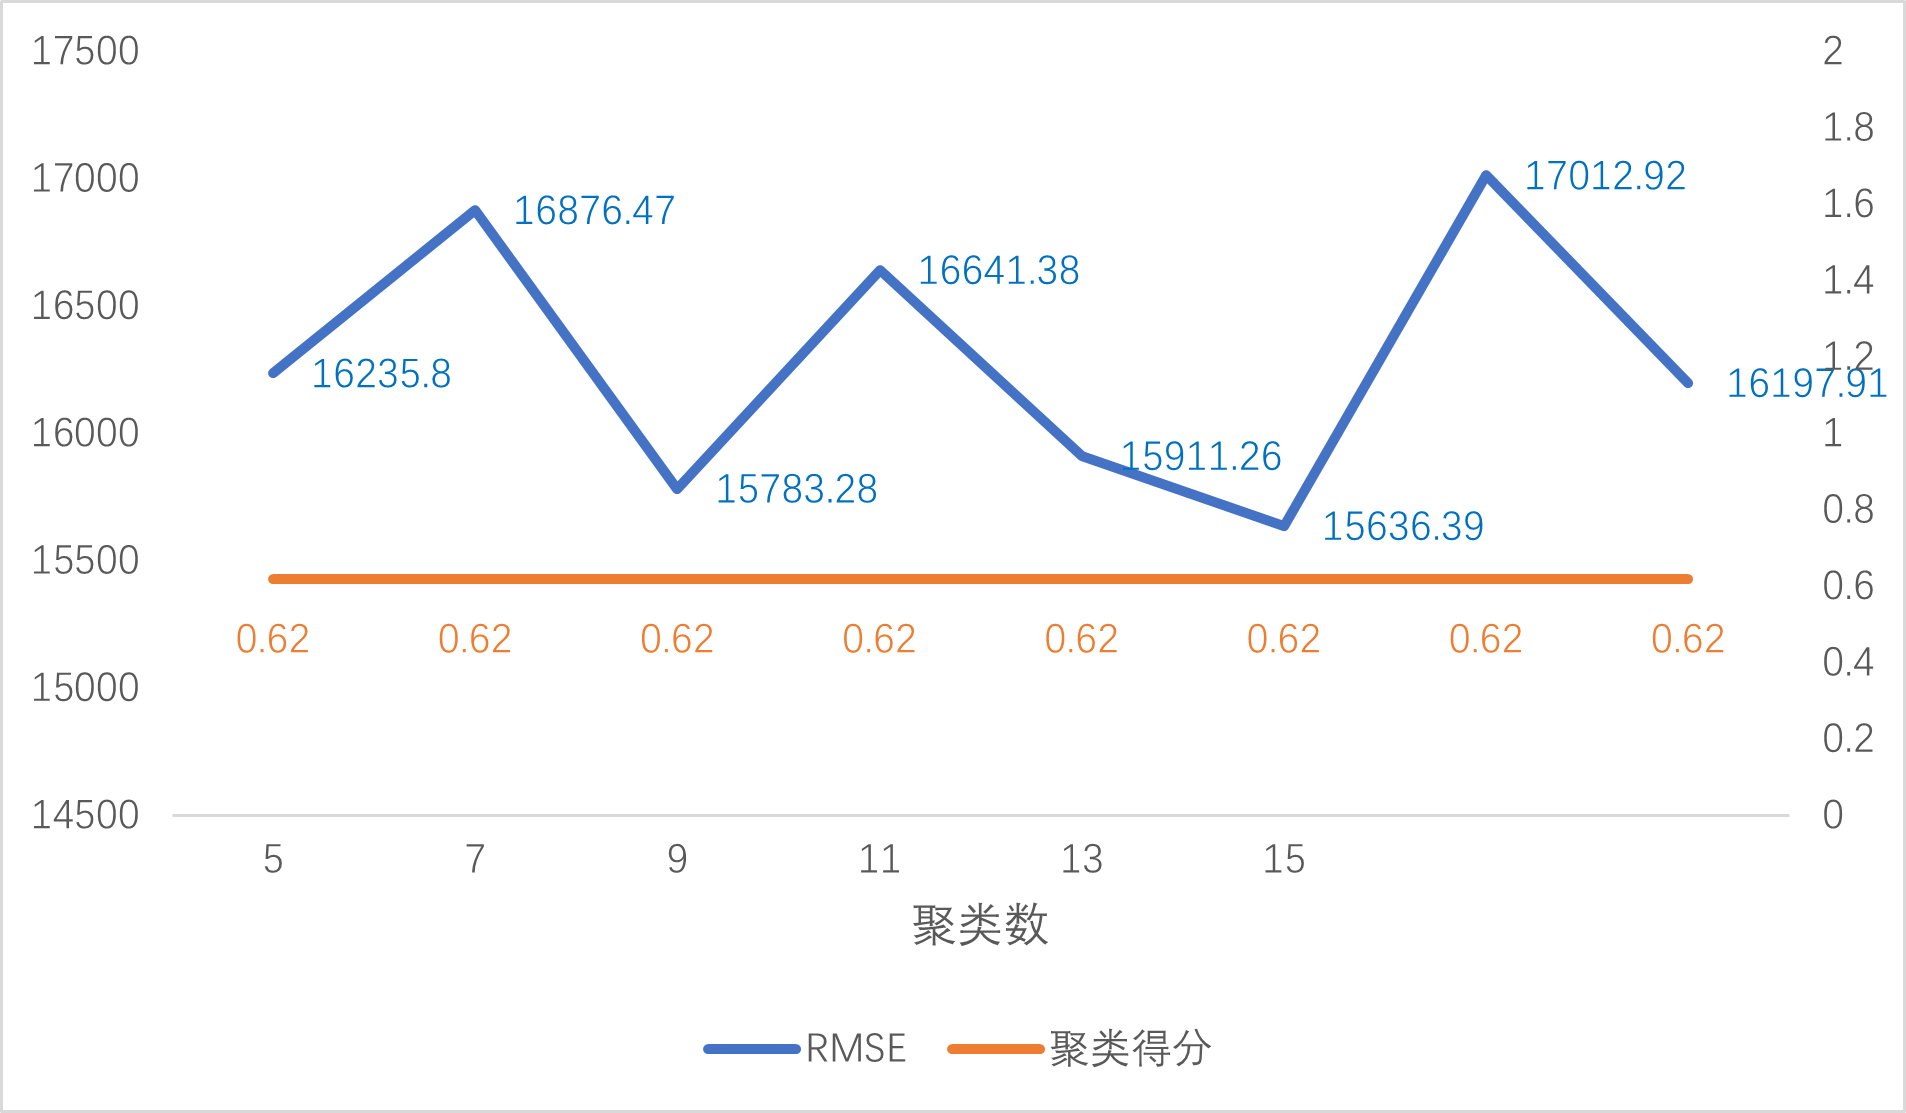
\includegraphics[width = 0.8\linewidth]{figures/7.12.png}
    \caption{特征数量灵敏度}
    \label{fig:feature}
\end{figure}
从我们的结果中可以看出,特征数量k的选择对于聚类得分并没有明显的影响,但是对于模型预测能力有一定的影响,本文选择的特征数为k=10,处于一个较优的配置,这也说明了本文参数选择的正确性,带来了比较好的模型性能。
\subsection{模型优缺点分析}
\subsubsection{模型优点}
\begin{enumerate}
    \item 本文在问题一中首先将血肿扩散的条件进行符号化,根据条件构建了一个优化后的集成模型进行病人血肿扩散风险的预测,同时考虑了变量之间的冗余性,针对影响较高的变量进行建模,高效精准地完成了风险地评估。相较于单一的模型具有更好的精度和更强的泛化能力,达到了99\%的预测精度。
    \item 本文在问题二中,对水肿发生时间和水肿体积大小进行建模。考虑到同一个发生时间可能会对应多个水肿体积大小,本文同时考虑了绝对时间(当前的治疗时间)和相对时间(发病到就医的时间)。并采用机理建模(混合精度模型)和网络建模(双向LSTM模型)相结合的方式,对水肿体积和残差进行建模,结果表明,这一建模方式能够有效应对一对多的数据分布问题。采用聚类的方法细分病患群体进一步提升了模型的预测性能,灵敏度分析的结果也表明本文的模型和超参数选择是鲁棒且高效的。
    \item 本文在问题三中对首次就医和多次就医数据的90天mRS进行建模。同时考虑了水肿和血肿的影像数据,并结合病人的群体特征进行建模,首次和多次数据的拟合精度在测试集上达到了55\%和97.5\%,在训练集上达到了87\%和99\%,并根据我们的模型结果对相应的群体提供了接受治疗的参考意见。
\end{enumerate}


\subsubsection{模型缺点}
\begin{enumerate}
\item 本文在问题二中,受限于因变量的选取,尽管采用绝对和相对时间变量,模型预测的RMSE仍然较大,还存在着数据一对多的问题。
    \item 本文在问题三中,仅使用首次就医数据对于90天mRS的性能仍然有一定的提升空间。可以在未来继续集成或者设计针对性的模型。
\end{enumerate}
    
    

% \subsection{模型推广}




%参考文献   手工录入
%\begin{thebibliography}{9}%宽度9
% \bibitem{bi        b:one} ....
% \bibitem{bib:two} ....
%\end{thebibliography}

%采用bibte        x方案
\clearpage
\bibliographystyle{gmcm}
\bibliography{reference}


\clearpage
%附录
\appendix

\section{附录}
附录中主要包含了核心的可执行的python代码,处理后的数据和所有代码(包括灵敏度分析和绘图代码)打包在补充材料中。
\subsection{问题一第一小问}
\lstinputlisting[language=python]{code/q1_a.py}
% \begin{appendices}
% %\setcounter{page}{1} %如果        需要可以自行重置页码。
\subsection{问题一第二小问}
\lstinputlisting[language=python]{code/q1_b_model.py}

% \subsection{问题二第一小问}
% \lstinputlisting[language=python]{code/q2_a.py}
% \end{appendices}
\subsection{问题二第二小问}
\lstinputlisting[language=python]{code/q2_b.py}

\subsection{问题二第三小问}
\lstinputlisting[language=python]{code/q2_c.py}

% \subsection{问题二第四小问}
% \lstinputlisting[language=python]{code/q2_d.py}

% \subsection{问题三第一小问}
% \lstinputlisting[language=python]{code/q3_a.py}

\subsection{问题三第二小问}
\lstinputlisting[language=python]{code/q3_b.py}

% \subsection{问题三第三小问}
% \lstinputlisting[language=python]{code/q3_c_pearson.py}
\end{document}
